% !TEX root =single_chapter_intro.tex
\chapter{Introduction}
\label{chap:intro}

\lettrine[lines=4]{F}{or} millennia mankind has watched and studied the night sky. Apart from planets and comets it appeared an immutable canvas on which the stars rested. It comes as no surprise that for ancient civilizations supernovae (which were very rare events, occurring only every few centuries ) were interpreted as important omens as they broke the paradigm of the unchanging night skies. As these events are so rare their origin remained a mystery until the middle of the last century. \citet{1934PNAS...20..254B} suggested that "the phenomenon of a super-nova represents the transition of an ordinary star into a body of considerably smaller mass". For the last 85 years the "supernova-branch" in astronomy has been developing. There have been many advances, but there are still many unknowns. This work addresses two subfields of supernovae: The unsolved progenitor problem for Type Ia Supernovae as well as quantifying the nucleosynthetic yield and energies of Type Ia supernovae.


\section{Ancient Supernovae}
\label{sec:ancientsn}

One of the earliest recorded supernovae is \sn{185}{}. It first appeared in December of 185 and was visible (however fading) till the August of 187. The main record is the \textit{Houhanshu} \citep{2006ChJAA...6..635Z} which had a described it to be close to $\alpha$ \textit{cen}. Follow-up in modern times have revealed a supernova remnant in a distance of roughly 1\,kpc near the $\alpha$ \textit{cen} \citep{2006ChJAA...6..635Z}. SN185 is often named as the oldest written record of a supernova, this is however sometimes contested as it is still not completely clear if the so called "guest star" was a comet or a the supernova.

The oldest undisputed record of a supernova is \sn{1006}{}, which also coincides with the brightest ever recorded supernova.  It was observed worldwide by asian, arabic and european astronomers. \citet{1965AJ.....70..105G} gives a good summary of the observations and interpretation given by these ancient observers. Ali ibn Ridwan was an Egyption astronomer who recorded the appearance of \sn{1006}{}. He wrote in a comment on Ptolemy's Tetrabiblos: ``\textit{I will now describe for you a spectacle that saw at the beginning of my education. This spectacle appeared in the zodiacal sign Scorpio in opposition to the sun, at which time the sun was in the 15th degree of Taurus, and the spectacle in the 15th degree of Scorpio. It was a large spectacle, round in shape and its size 2.5 or 3 times the magnitude of Venus. Its light illuminated the horizon and twinkled very much. $\dots$ This apparition was also observed at the time by (other) scholars just as I have recorded it.}''

The next supernova happened only 50 years after \sn{1006}{} in 1054. 
\sn{1054}{}, like \sn{1006}{}, was observed by many astronomers. One of the records is are petroglyphs in the Chaco Canyon (see Figure \ref{fig:sn1006_chaco}) and was determined to have been produced around the time of the SN1054 explosion. It is still debated if SN1054 was the inspiration of the painting or the inspiration came from the passing of Hailey's comet in 1066. 
More than 900 years later \cite{1968Sci...162.1481S} detected a pulsar in the center of SN1054. This was the first time that the stellar remnant of a supernova was found.

\sn{1181}{} is a Galactic supernovae that has been mentioned in eight different texts by Chinese and Japanese astronomers. 3C58, a pulsar found in \sn{1181}{}, is suggested as the neutron star remnant of this stellar explosion. 



\begin{figure}[htbp] %  figure placement: here, top, bottom, or page
   \centering
   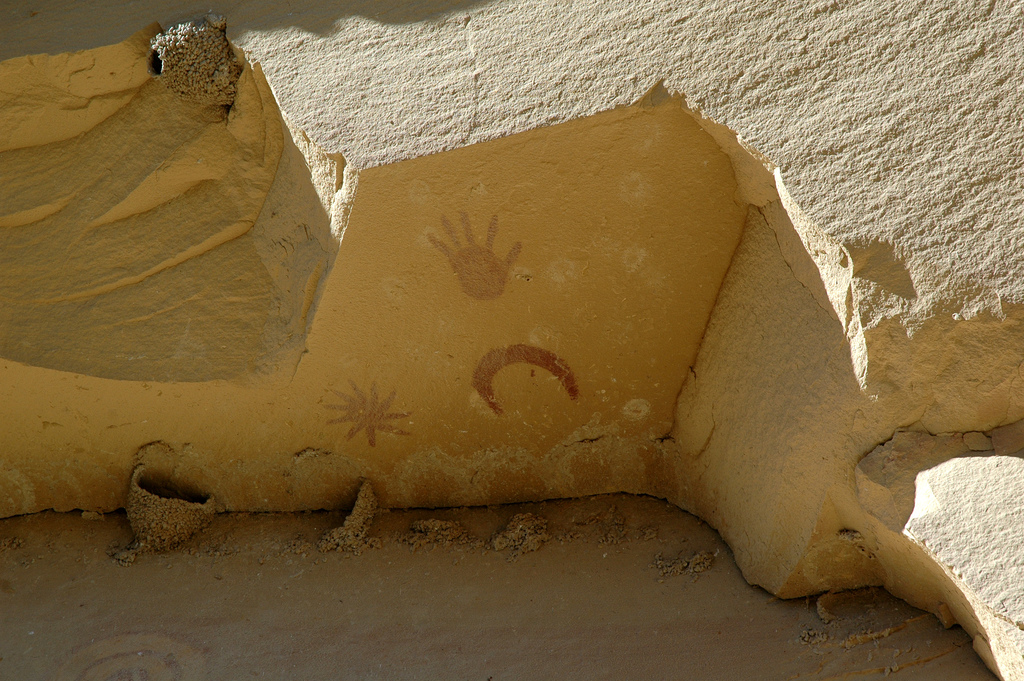
\includegraphics[width=\textwidth]{chapter_intro/plots/Chaco_canyon_pueblo_bonito_petroglyphs.jpg} 
   \caption{Chaco canyon petroglyphs show a hand, a moon and a bright celestial object. This could be SN1054 but it is ambiguous. (Source Wikipedia/ Photographer jamesdale10/ Creative Commons license)}
   \label{fig:sn1006_chaco}
\end{figure}


The supernova of 1572 has been reported by many astronomers. The most famous record, however, stems from the danish astronomer Tycho Brahe \citep{1602QB41.B73.......}. The supernova was observed from November 1572 and monitored till March 1574 when it faded from visibility. Figure \ref{fig:sn1572_tycho_chart} shows the original chart produced by Tycho Brahe which shows the supernova in the constellation of Cassiopeia. Nearly 400 years later \citet{1952Natur.170..364H} discovered the radio emissions from the remnant of the SN1572. 


32 years after the discovery of SN1572 Kepler and others observed SN1604 \citet{kepler1606} . The supernova remained visible for about 18 month. 

\begin{figure}[htbp] %  figure placement: here, top, bottom, or page
   \centering
   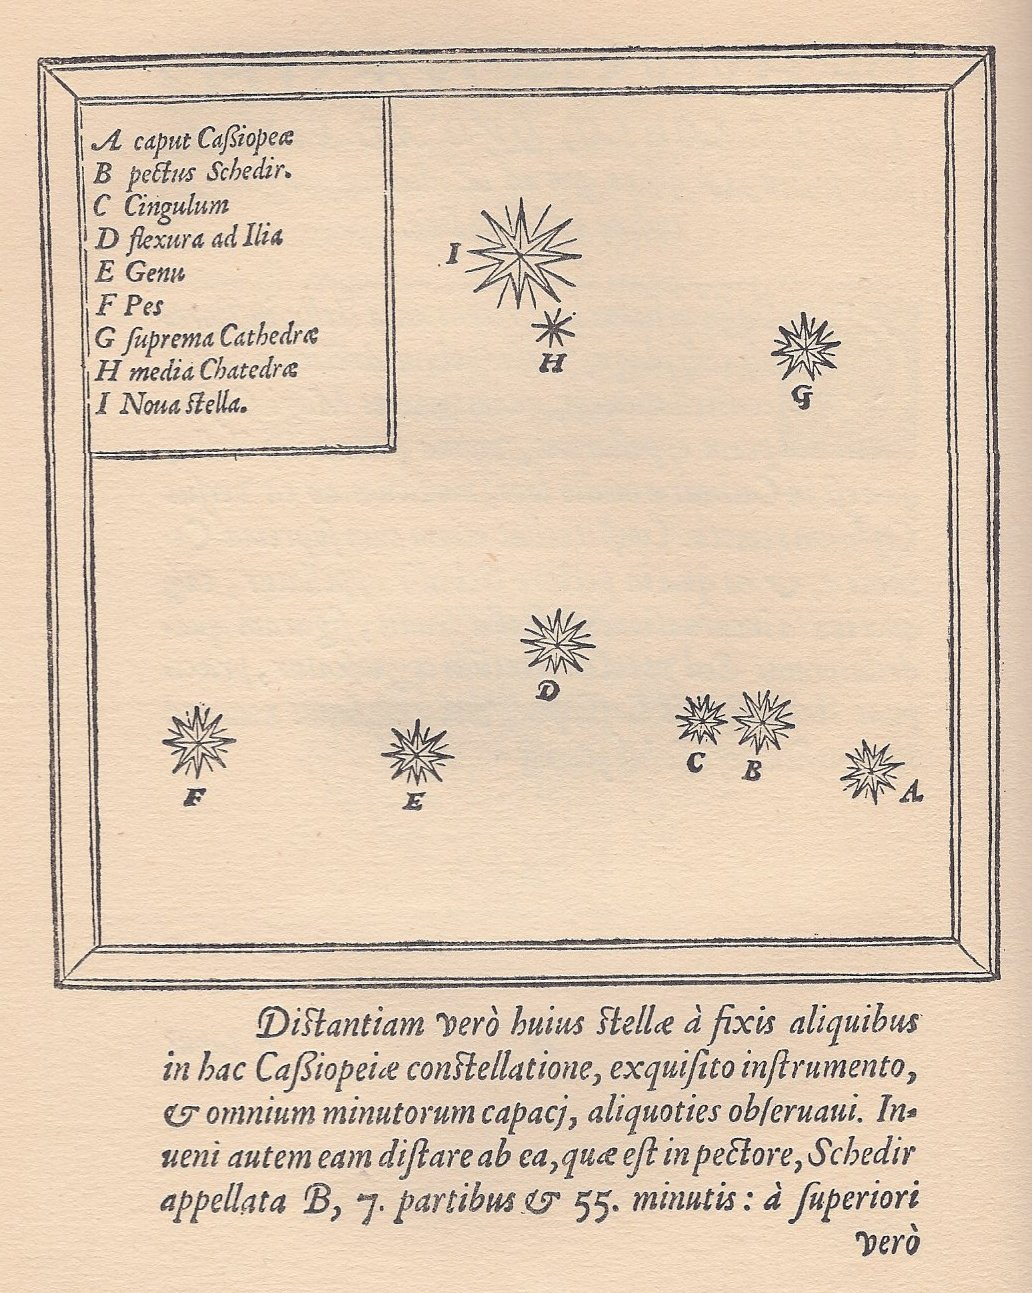
\includegraphics[width=0.7\textwidth]{chapter_intro/plots/Tycho_Cas_SN1572.jpg} 
   \caption{\textit{"I have indeed measured the distance of this star from some of the fixed stars in the constellation of Cassiopeia several times with an
exquisit (optical) instrument, which is capable of all the fine details of measurement. I have further detected that it
(the new star) is located 7 degrees and 55 minutes from the star at the breast of the Schedir designated by B."} translation kindly provided by Leonhard Kretzenbacher}
   \label{fig:sn1572_tycho_chart}
\end{figure}

All of the ancient supernovae were observed only by the naked eye. Even in an era of 10-meter telescopes the records of these explosions remain useful.

\section{Modern day supernova observations and surveys}
\label{sec:surveys}

The era of modern day supernova observations started with the discovery of \sn{1885}{}. \sn{1885}{} (also known as S Andromedae) was first spotted by Isaac Ward in Belfast in August of 1885 \citep{1885AN....112..360H} and was visible till February 1886. 
More than 50 years later \citet{1934PNAS...20..254B} coined the term supernova and established the difference between common novae and supernovae. \citet{1934PNAS...20..254B} also suggested that these luminous events are caused by the death of stars. 

In order to understand the phenomenon of the supernova better, Zwicky began a supernova search with the 18-inch Schmidt telescope . Zwicky found several supernovae which in turn inspired Minkowski to classify these supernovae by their spectra \citet{1941PASP...53..224M}. 
He categorized the 14 known objects into two categories. Those without hydrogen he called 'Type I', those with hydrogen he called 'Type II' (see section \ref{sec:sn_classification} for a more detailed description about classification).

With the advent of affordable computing in the 1960s the first computer controlled telescopes were build. The 24-inch telecope was built by the Northwestern University and was deployed in Corralitos Observatory in New Mexico \citep{1975PASP...87..565C}. This search lead the way in computer controlled discovery and many later surveys would employ a similar design.

The Cal\'{a}n/Tololo supernova survey \citep{1993AJ....106.2392H} ushered in the era of the modern automated supernova surveys in the 1990's. They provided a set of high-quality light curves and spectra of moderately distant $(0.01 < z < 0.01)$ supernovae.

The Leuschner Observatory Supernova Survey began in 1992 followed shortly by the Berkeley Automatic Imaging Telescope (BAIT). These searches resulted in 15 supernovae by 1994 \citep{1994AAS...185.7905V}. One of the most well known discoveries is \sn{1994}{D}. This supernovae was observed with the Hubble Space Telescope and resulted in an image that is widely used today.

Having started in 1988 the supernova cosmology project (henceforth SCP) is the longest running supernova search which is still active today. Their main sample for the famous paper \citep{1999ApJ...517..565P} used the CTIO 4m telescope for discovery and many other telescopes for follow-up.

The High-Z team used the CTIO 4m telescope for discovery and follow-up of supernovae \citep{1998ApJ...507...46S}. Independently to SCP they discovered the accelerated expansion of the universe \citep{1998AJ....116.1009R}.


The Lick Observatory Supernova Search (LOSS) using the Katzman Automatic Imaging Telescope (KAIT) is one of the most successful supernovae searches. By the year 2000 it had found 96 supernovae \citep{2001ASPC..246..121F}. 

After the turn of the millennium and following the discovery of the accelerated expansion of the universe a variety of groups started searching for supernovae and other transients. Among them were ``The Equation of State: SupErNovae trace Cosmic Expansion (ESSENCE)''-project \citep{2002AAS...201.7809G} and the Supernova Legacy Survey (SNLS) \citep{2003AAS...203.8209P}. Both these programs have either finished or are close to finishing. 

Specialised surveys like the Nearby Supernova Factory \citep{2002SPIE.4836...61A} and the Higher-z survey \citep{2004ApJ...613..200S} focused on a certain redshift range to obtain data on supernovae.

In recent years a multitude of large sky surveys has started (or are just about to). Some of these focus exclusively on transients and supernovae \citep[e.g. PTF;][]{2009PASP..121.1334R}, whereas others like PanSTARRS \citep{2004SPIE.5489...11K} and SkyMapper \citep{2007PASA...24....1K} have a transient/supernova component. 
Upcoming surveys like the LSST \cite{2006AAS...209.8604P} and the space-based GAIA mission \cite{2001A&A...369..339P} will provide unprecedented detail about current supernovae as well finding several new classes of transients.

In addition to the search in the optical new high-energy instruments like BATSE surveyed the sky from the beginning of the 1990's in \gammaray s. \citet{1992Natur.355..143M} showed that \grb s due to their isotropic distribution are events at cosmological distances rather than coming from our own Galaxy. 

The Beppo-SAX satellite played a crucial role in resolving the origins of \grb s. The data from this mission was used to establish the connection between some \grb s and supernovae, the most famous example being GRB980425/\sn{1998}{bw} \citep{1998Natur.395..670G}.

Among other discoveries the Hete-2 mission established a new class of transients called \xray-flashes. These new objects are thought to be similar to  \grb s in the physical nature but much less energetic \citep{2004ApJ...601L.119Z}.  

It was followed by the SWIFT telescope which provides, in addition to the \gammaray-detector, an X-Ray telescope and UV/Optical telescope. It has been very successful at finding \grb s and providing targets for follow-up.

Almost all of the information about the universe we have deduced from observations of electro-magnetic waves. There are different physical phenomena which are much harder to observe than the electro-magnetic spectrum.

Gravitational waves, predicted by the theory of general relativity  \cite{1918SPAW.......154E}, might provide us with another insight into supernovae. The most advanced detector today \cite[LIGO][]{1992Sci...256..325A} has up till now not unambiguously detected gravitational waves. The sensitivity for this instrument is probably not low enough to detect these waves. Future instrumentation, like the impressive LISA-project \citep{1994ESAJ...18..219J}, are sensitive enough to detect the predicted gravitational waves. In the supernova field LISA might give us an estimate on the number of in-spiralling white dwarfs, which are suggested as progenitors of \sneia.

\citet{1987PhRvL..58.1494B,1987PhRvL..58.1490H,Alekseev:1988gp} reported on neutrino detections from the very nearby supernova SN1987A. This was the first and last time that neutrino emission from a supernova was measured. New more sensitive detectors like ICECUBE \citep{2008ICRC....4..835K} will hopefully enable us to do neutrino observations of more distant events.

For now the optical observations of supernovae provide the bulk of observations of these transients. Hopefully future instruments and capabilities will give us panchromatic observations as well as measurements from gravitational waves and particle fluxes. 
This will hopefully help to unlock more of the secrets of these still mysterious supernovae.

\section{Observational Properties of Supernovae}

\subsection{Supernova classification}
\label{sec:sn_classification}

The classification of supernovae started in the 1941 when Minkowski realized that there seem to be two main types \citep{1941PASP...53..224M}. Those containing a hydrogen line (6563 \AA) he called Type II supernovae and those showing no hydrogen he called Type I supernovae.  

\begin{figure}[htb] %  figure placement: here, top, bottom, or page
   \centering
   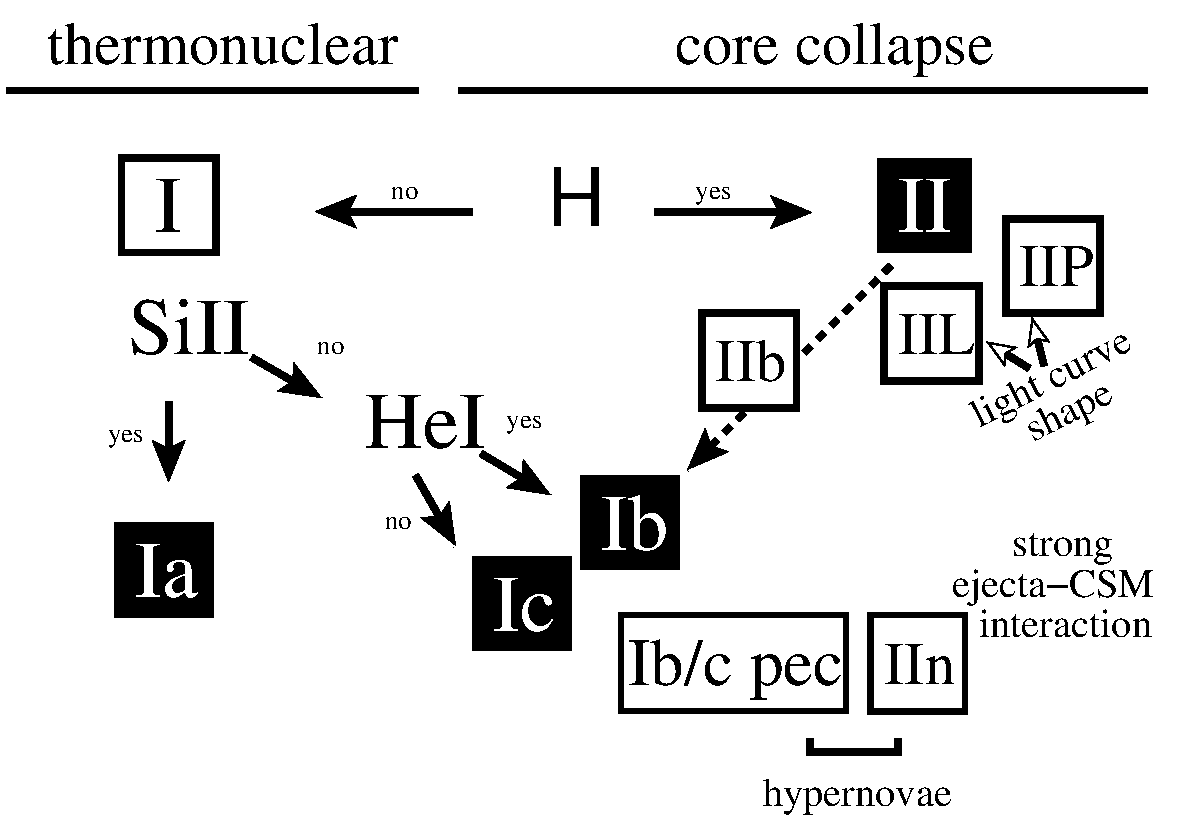
\includegraphics[width=.7\textwidth]{chapter_intro/plots/sn_classification.pdf} 
   \caption{}
   \label{fig:sn_classification}
\end{figure}

This basic classification has remained to this day, however the two main classes branched into several subclasses.
During the 1980s the community discovered that most \sneia\ showed a broad Si II line at 6130 \AA. There was, however, a distinct subclass of objects that lacked this feature. These Silicon-less objects were then subclassed further into objects that showed helium -- now known as Type Ib --  and those that did not were called Type Ic \citep[see spectra in Figure \ref{fig:sn_classification};]{1987ApJ...317..355H, 1986ApJ...306L..77G}. The classical Type I supernova was renamed to Type Ia. 

\begin{figure}[htb] %  figure placement: here, top, bottom, or page
   \centering
   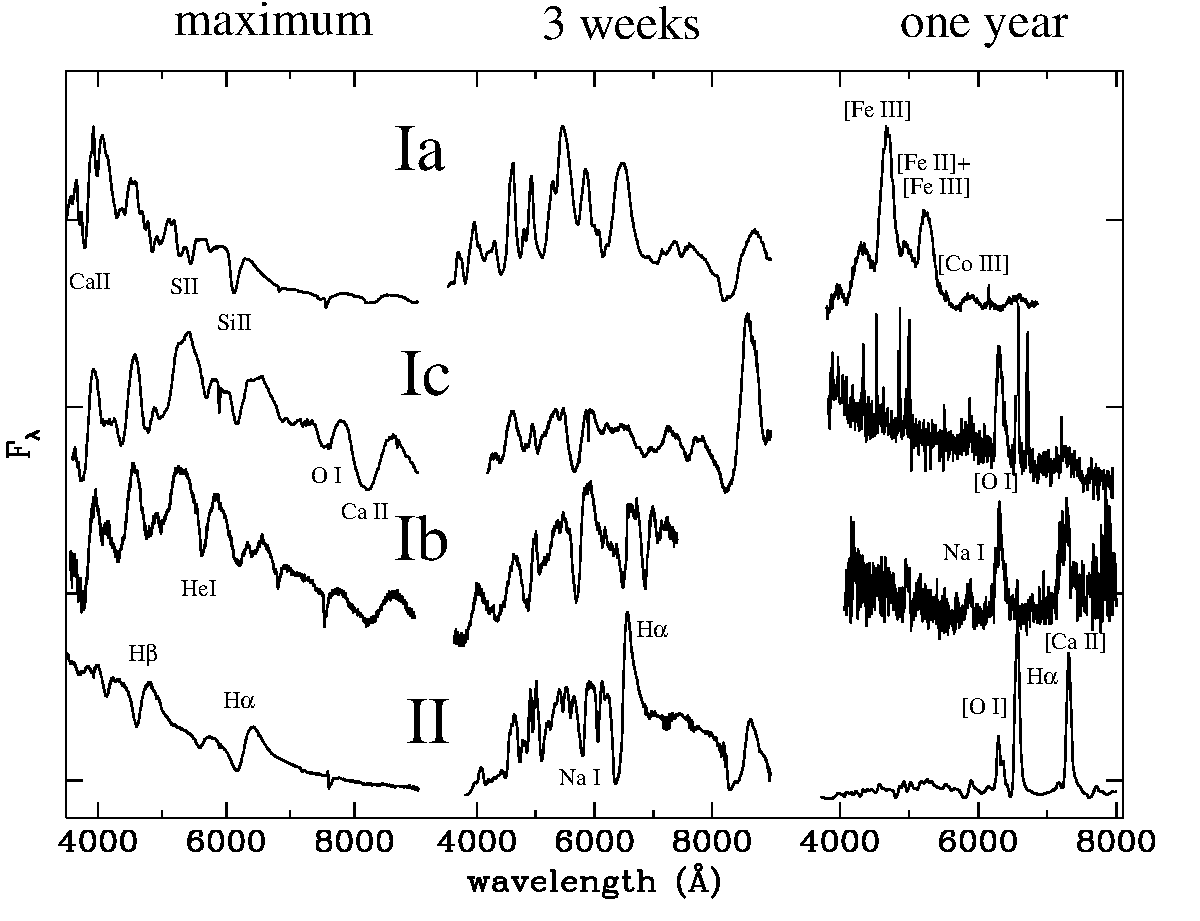
\includegraphics[width=0.7\textwidth]{chapter_intro/plots/sn_class_spectra.pdf} 
   \caption{example caption}
   \label{fig:sn_class_spectra}
\end{figure}

%This classification only uses static spectral features. In recent years, however, there has been a push towards also using the lightcurve and spectral evolution as classification parameters. \citet{2005ApJ...623.1011B} provide an overview of this subclassing of \sneia\ and suggest that there are two distinct subclasses of \sneia. As a parameter for this further partitioning they use the velocity measured from the Si II feature at 6130 \AA. Those with a relatively fast decline in this radial velocity they call \hvg\ (high velocity gradient) those with a slow decline rate are named \lvg\ (low velocity gradient). 

\sneia\ show a low intrinsic scatter in peak luminosity. Only in the past two decades have we been able to explore the finer details of the \sneia-class.
Most objects have a small brightness scatter and are referred to as ``Branch''-normal \citep{1993AJ....106.2383B}. 
There however seem to be two distinct subclasses with extreme luminosities. The overluminous class we call 91T\,s after the bright supernova \sn{1991}{T} \citet{1992AJ....103.1632P, 1994ApJ...434L..19S} and the faint 91bg\,s named after the faint \sn{1991}{bg}\ \citep{1992AJ....104.1543F}.  As a further characteristic the community uses the velocity inferred from the Si II feature at 6130 \AA.
Faint supernovae are fast decliners both in velocity as well as luminosity \citet{2005ApJ...623.1011B}. The bright supernovae do not seem to have such a preference. 
A third subclass named after \sn{2002}{cx}\ \citep{2003PASP..115..453L} seems to contradict this theme. They decline slow and are faint. This subclass also shares spectral traits with the overluminous 91T\,s.

\citet{2011MNRAS.412.1441L} have tried to measure the fraction of these different subclasses from the Lick Observatory Supernova Search (LOSS). Figure \ref{fig:ia_fracs} shows the fraction of the different subclasses that would be expected from a purely magnitude limited search. 

\begin{figure}[htbp] %  figure placement: here, top, bottom, or page
   \centering
   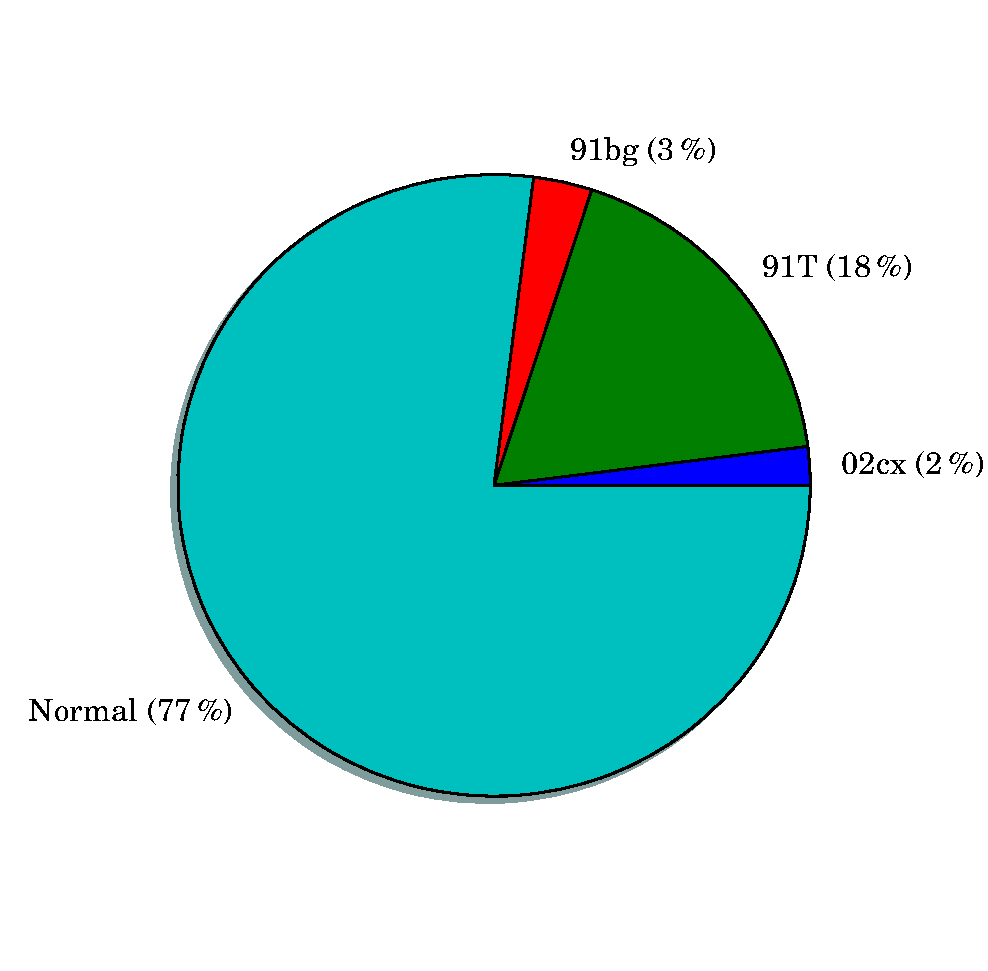
\includegraphics[width=0.7\textwidth, trim=0 2.5cm 0 0cm]{chapter_intro/plots/plot_ia_fracs.pdf} 
   \caption{Estimated fractions for different \snia-classes for a purely magnitude limited search. Adapted from \citet{2011MNRAS.412.1441L}}
   \label{fig:ia_fracs}
\end{figure}

In summary, although there are several different subclasses, the \snia\ as a class itself is relatively homogenous when compared to the different \sneii.

\begin{figure}[htbp] %  figure placement: here, top, bottom, or page
   \centering
   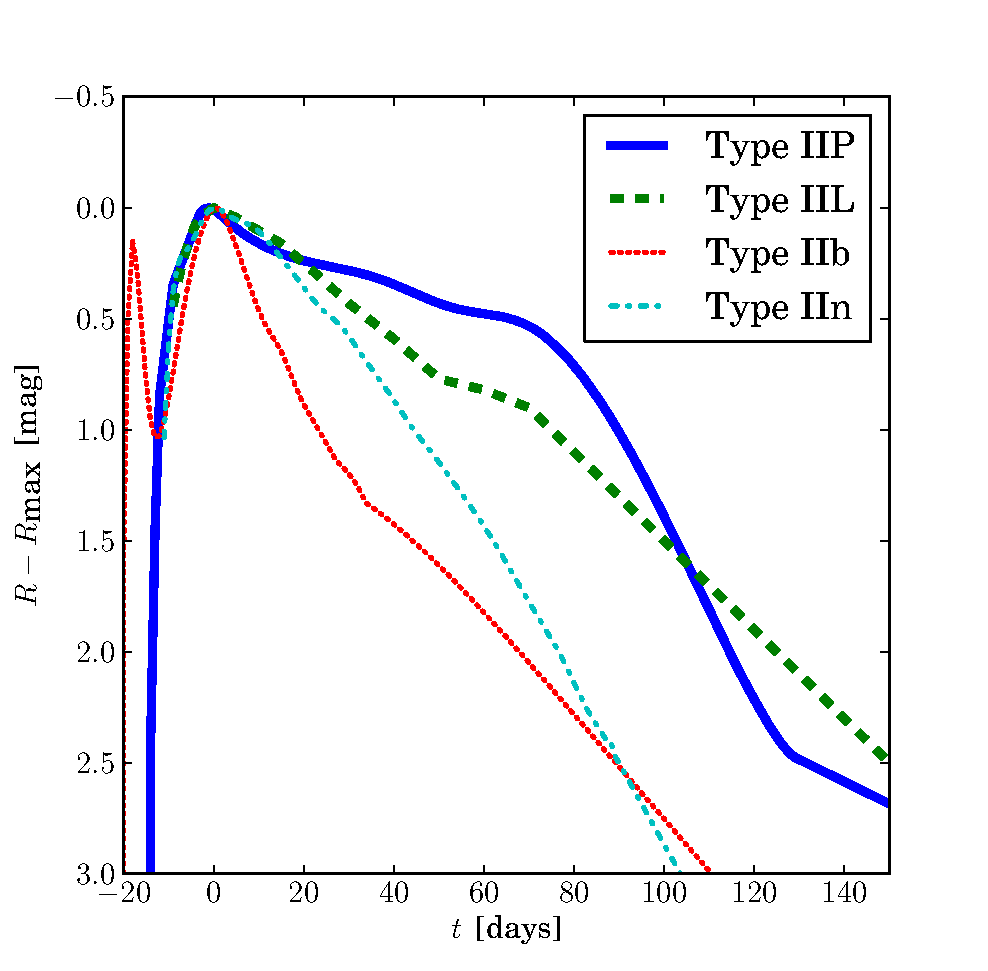
\includegraphics[width=0.7\textwidth]{chapter_intro/plots/plot_li11_lc_type2.pdf} 
   \caption{Lightcurve data taken from \citet{2011MNRAS.412.1441L} templates. The time is relative to maximum light and the magnitude is the difference between maximum  }
   \label{fig:snii_lc}
\end{figure}

\sneii\ span large ranges in observable parameters. We can divide the main class into four main subclasses. Type II Plateau Supernovae \citep[henceforth \sniip;][]{1979A&A....72..287B} have a relatively flat light curve after an initial maximum (see Figure \ref{fig:snii_lc}). In contrast the Type II Linear Supernovae \citep[henceforth \sniil;][]{1990MNRAS.244..269S} have a rapid linear decline after the maximum. The third subclass is the narrow-lined Type II Supernova (henceforth \sniin) which is characterized by narrow emission lines, which are thought to come from interaction with the \csm. 
Finally the Type IIb supernovae (henceforth \sniib) show strong hydrogen lines in their early spectrum, but evolve to become spectroscopically to be more like Type Ib supernovae with no hydrogen lines but strong Silicon and Helium lines. An interesting feature is the second maximum observed in the \sniib \sn{1993}{J} (Figure \ref{fig:snii_lc}). It is believed that many more \sniib s exhibit this feature but are not detected early enough \citep[this feature has also been seen in SN2008D a  \snib][]{2008Natur.453..469S, 2009ApJ...702..226M}. 

Figure \ref{fig:ii_fracs} shows the estimated fractions of the different \sneii\ that would be expected from a purely magnitude limited survey.

\begin{figure}[htbp] %  figure placement: here, top, bottom, or page
   \centering
   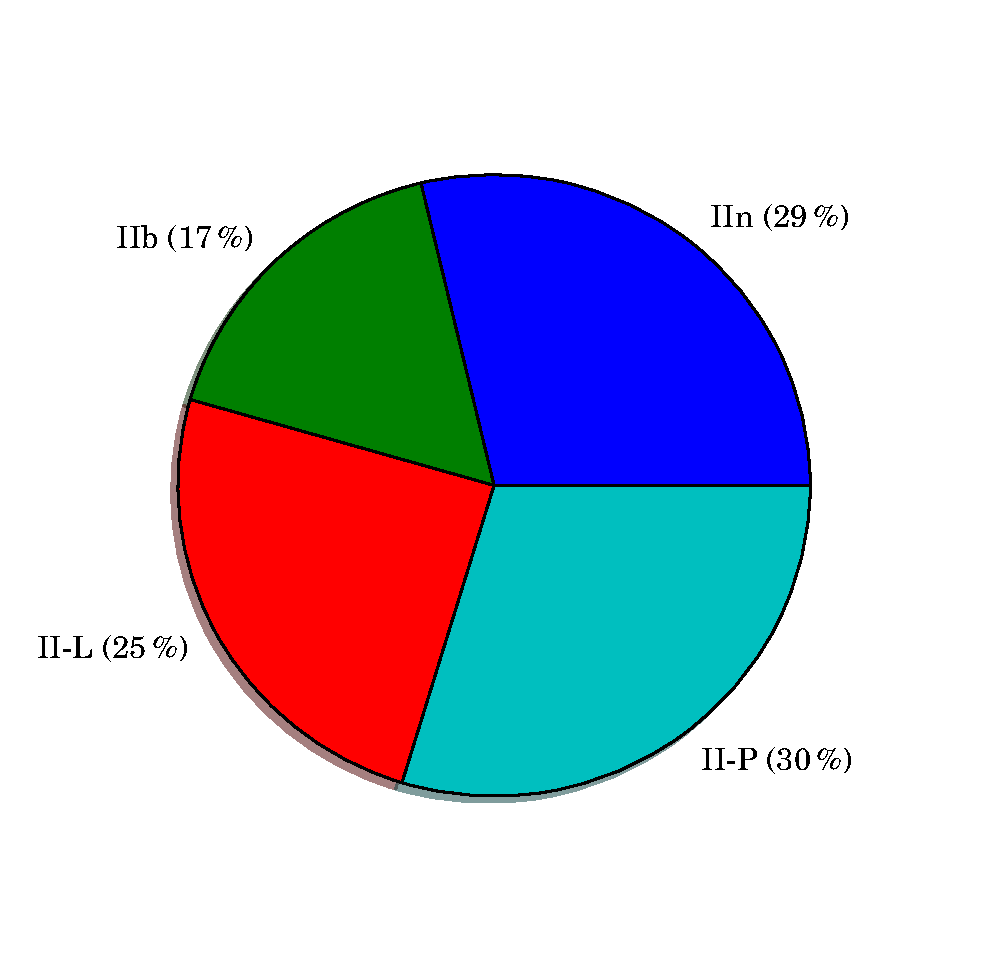
\includegraphics[width=0.7\textwidth, trim=0 2.5cm 0 0cm]{chapter_intro/plots/plot_ii_fracs.pdf} 
   \caption{Estimated fractions for different \snii-classes for a purely magnitude limited search. Adapted from \citet{2011MNRAS.412.1441L}}
   \label{fig:ii_fracs}
\end{figure}


Unlike the \sneia\ there are numerous intermediate objects among these three basic classes and some peculiar objects.


For a more comprehensive review of the classification of supernovae the reader should consult \citet{2003LNP...598...21T} and \citet{2007AIPC..937..187T}.

\subsection{Supernova rates}
\label{sec:sn_rates}
The observed supernova frequency carries important information about the underlying progenitor population. In this section we will concentrate more on \sneia-rates but will mention \sneii\ and \sneibc where applicable.

\citet{1938ApJ....88..529Z} was the first work that tried to measure the supernova rate. By monitoring a large number of fields monthly, they arrived at a supernova rate by merely dividing the number of supernova detection by the number of monitoring time and galaxies. This crude method resulted in a rate of one supernova per six centuries. 

Over time many improvements were made to this first method. The rate was divided by galaxy morphological class as well as different supernova types. To normalise these quantities were then defined by the supernova rate as number of events per century per $10^{10}$\,\lsun\ \citep[e.g.][]{1991ARA&A..29..363V,1994ApJS...92..487T}. 

In recent years, however, rate measurements have been in relation to star formation rather than galaxy luminosity (\sn\ per century per $10^{10}$\,\msun).  The community \citep[e.g.][]{2005A&A...433..807M} have switched to the use of infrared photometry for the galaxy as it is thought to better represent star-formation rate then B-Band photometry \citep{2003A&A...410...83H} which had been used previously. 
\begin{figure}[htbp] %  figure placement: here, top, bottom, or page
   \centering
   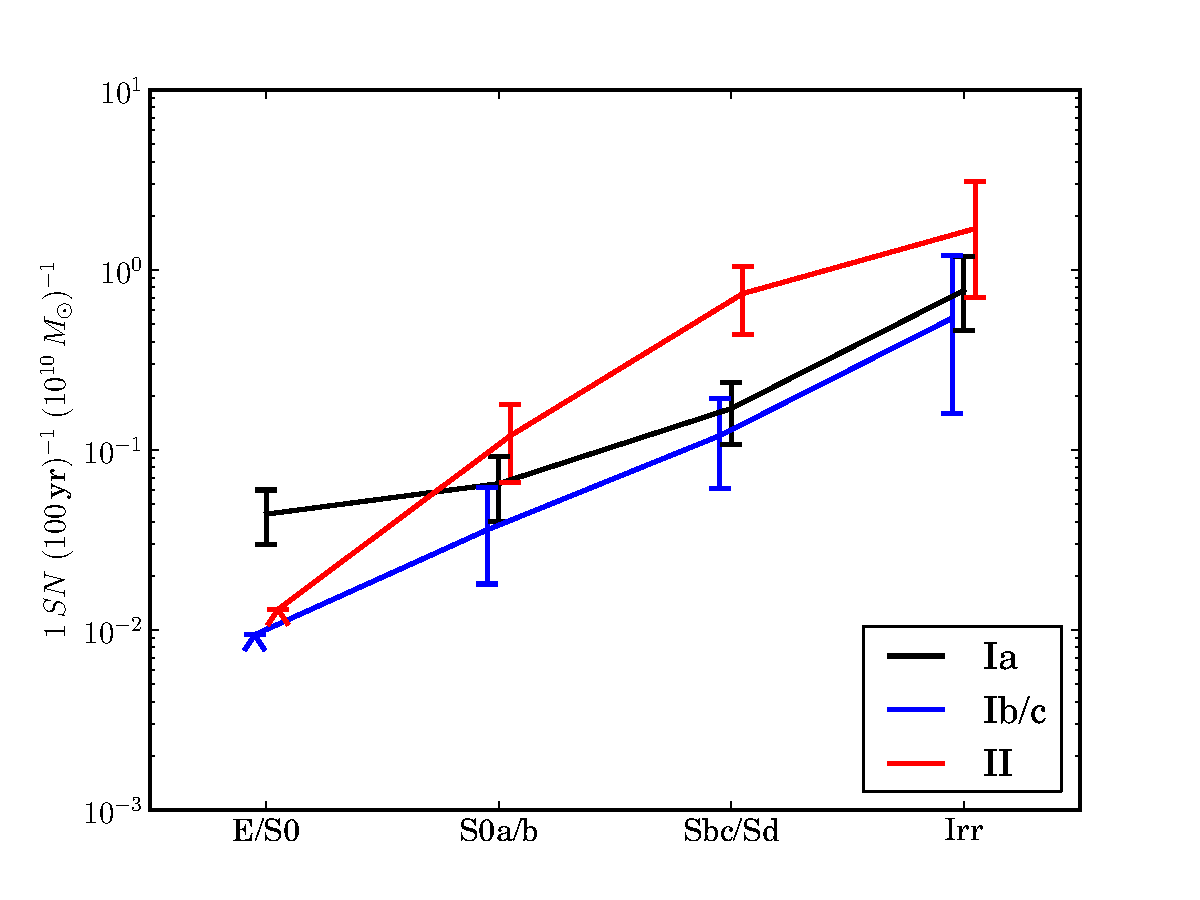
\includegraphics[width=\textwidth]{chapter_intro/plots/snrates_mannucci05.pdf} 
   \caption{The plot shows the estimated supernova rate per unit mass in different galaxy morphologies \citep{2005A&A...433..807M}. There have been no detections of \sneibc\ and \sneii\ in old elliptical galaxies which suggests that these types only occur in galaxies with recent star-formation.}
   \label{fig:snrates_mannucci05}
\end{figure}

Figure \ref{fig:snrates_mannucci05} clearly shows that there is a strong connection between morphology and supernova rates. This suggest that \sneii\ and \sneibc\ come from populations with recent star formation, which implies massive stars as progenitor. \sneia\ occur both in old elliptical galaxies and young spirals. It seems the progenitors occur in both of these environments. This could hint that there are two main progenitor types one which occur soon after star-formation, whereas others take a long time between formation and explosion. The progenitors of \sneia\ are a highly debated topic (see Section \ref{sec:snia_progenitors}).

To address this issue several groups have tried to measure a \sneia-rate that is completely independent of galaxy morphology \citep[e.g.][]{2006MNRAS.370..773M, 2010ApJ...722.1879M}. This so called, delay time distribution (\dtd), measures the supernova rate over time following a brief outburst of star formation.
This technique requires a detailed knowledge of the star-formation history of these systems. Several new techniques are emerging that try to circumvent the intrinsically difficult task of determining star-formation for individual \sneia\ host galaxies \citep{2010MNRAS.407.1314M, 2010arXiv1010.5786B, 2008PASJ...60.1327T, 2010ApJ...722.1879M}.

Supernova rates and \dtd s are a great tool to constrain progenitors. New upcoming surveys will provide an abundance of supernovae and measurements of their environments.

\subsection{Light curves} 
Light curves give important insights into the physical reactions occurring during the evolution of the supernova. \cite{1982ApJ...253..785A} for example deduced from the light-curve shape that Type I supernova are eventually powered by the decaying \Co. 


\begin{figure}[htb] %  figure placement: here, top, bottom, or page
   \centering
   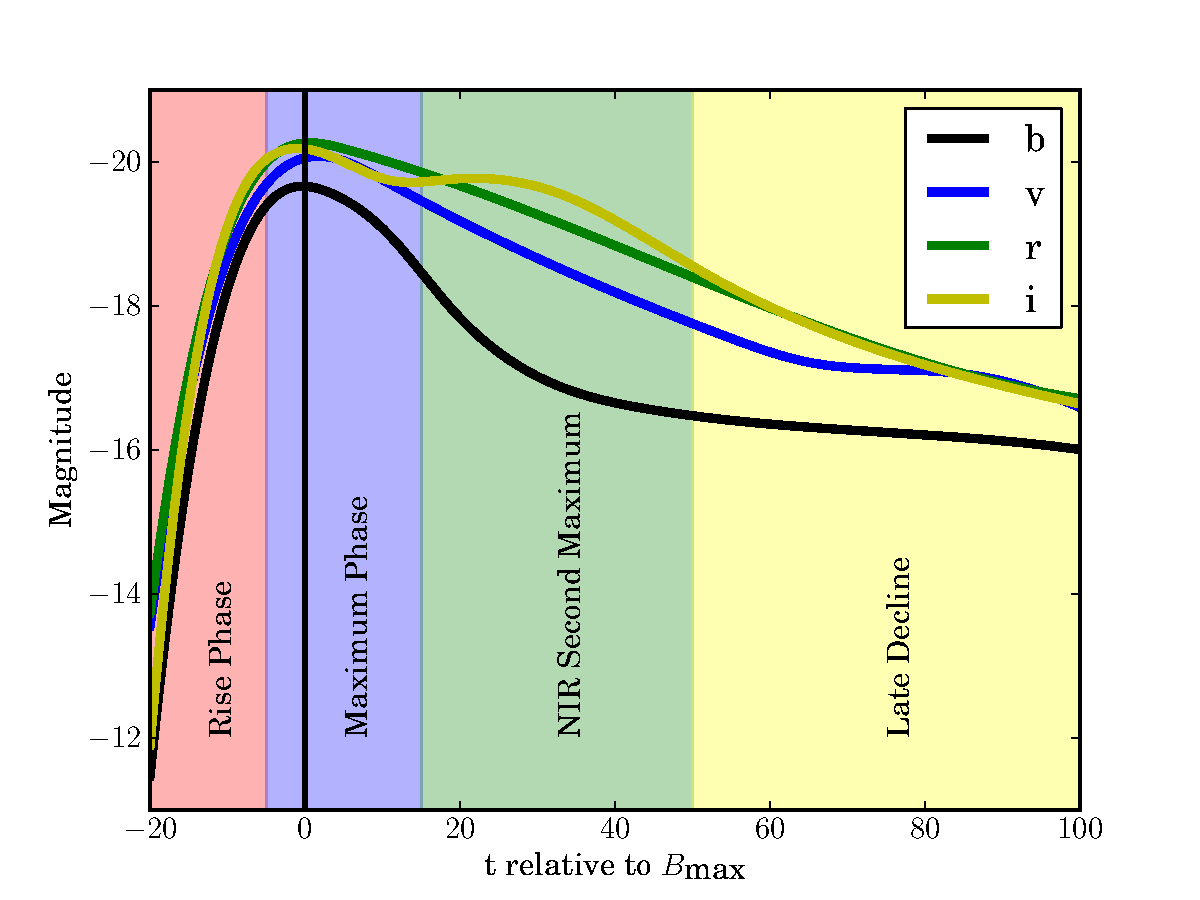
\includegraphics[width=\textwidth]{chapter_intro/plots/lightcurve_2002bo.pdf} 
   \caption{Lightcurves of SN 2002bo (data from ??)}
   \label{fig:lightcurve_2002bo}
\end{figure}

For \sneia\ the light curve can be divided in four different phases (see Figure \ref{fig:lightcurve_2002bo}). In the first phase the \sneia\  rises to the maximum brightness. Although only a small fraction of \sneia\ have been observed in that phase, one can determine the time of the explosion by approximating the very early phase of a \sneia\ with an expanding fireball. The luminosity of the fireball is 
\[L\propto v^2 (t+t_\textrm{r})^2 T\,,\]
where v is the photospheric velocity, T is the temperature of the fireball, t is the time relative to the maximum and $t_\textrm{r}$ is the rise time. A rise time of 19.5 days \citep{1999AJ....118.2675R} seems to fit most \sneia. 

The rise is very steep and the brightness increases by a factor of $\approx 1.5$ per day until 10 days before maximum. 

The \snia\ reaches the maximum first in the \nir\ roughly 5 days before the maximum in the B-Band \citep{2000MNRAS.314..782M}. 
During the pre-maximum phase the color stays fairly constant at B-V=0.1, but changes non-monotonically to B-V=1.1 30 days after maximum. 

The \snia\ starts to fade but  a second maximum is observed in the \nir\ \citep{2008ApJ...689..377W}.  \citet{2006ApJ...649..939K} has succesfully explained this by fluorescence of iron-peak elements in the \nir. 

At roughly 600 days after maximum the light curve begins ???? 1991t had a foreground dust??? (how late do light curves go; a comment would be nice here brian ;-) ) 

Arguably the most important use of light curves is their application in normalizing \sneia\ to standard candles (see Figure \ref{fig:normalized_lightcurve}). \citet[][]{1993ApJ...413L.105P} plotted the magnitude at maximum in different filters against the decline of the B-Band magnitude after 15 days (\dmb).  They found a strong linear relation with a very high correlation coefficient ($>$ 0.9). Dust extinction in the host is one of the major systematic problems and remains so to this day. 

\cite{1995ApJ...438L..17R} refined the method by using a linear estimation algorithm. This method would deliver a distance modulus by finding the offset between a template and the supernova lightcurve. They calibrated this method against a set of \sneia\ with known distances. 
Light curve fitting tools are still in active development \cite[e.g.][]{2007ApJ...659..122J, 2007A&A...466...11G}.

For description of lightcurves of \sneii\ please refer back to section \ref{sec:sn_classification}.


\subsection{Spectra} 

Spectra are much more detailed measurements of Supernovae than just lightcurves. They are however, observationally much more expensive. 

For all classes supernova spectra can be divided in two phases: the photospheric phase and the nebular phase.
In the photospheric phase, the spectrum can be very well approximated by a dense optically thick core which has a black-body radiating surface with an optically thin expanding ejecta above. Photons is often negligible in the ejecta. The ejecta rather reprocesses the radiation field coming from the central photosphere. 
In the case of \sneia\ the core consists mainly of decaying \Ni\ which produces the energy for the radiating photosphere. For \sneii\ the core mainly consists of ionized hydrogen.

As the supernova expands the photosphere recedes further into the core and the optically thin layer grows larger and larger. Once sufficiently expanded the entire SN ejecta becomes optically thin, which is known as the nebular phase. This phase is dominated by strong emission peaks and no continuum. 


\subsubsection{SNe Ia spectra}

\sneia\ spectra help us understand the physical processes in the thermonuclear explosion. 
Shortly after the explosion the ejecta is in homologous expansion.
The observed spectra are characterized by an underlying continuum - emitted from the photosphere -- and absorption features from the ejecta material above the photosphere. 
As time passes the photosphere recedes into the remnant and deeper layers of the exploded white dwarf become spectroscopically visible. Synthetic modelling of spectra is an important component to understanding \sneia\ and will be discussed in detail in Chapter \ref{chap:dalek}.

This time-variability in the spectra is used to conduct tomography on \sneia\ \citep{2005MNRAS.360.1231S, 2009MNRAS.399.1238H}.

Similar to light-curves the spectra have different phases. We will use the ``normal''-\snia\ \sn{2003}{du} to demonstrate the spectral evolution \citep{2011MNRAS.410.1725T}. 

\paragraph{Pre-Maximum Phase}
In the pre-maximum phase the spectrum shows very high velocities (up to 18 000 \kms). There is a relatively well defined pseudo-continuum with strong \pcygni-profiles of \ime s and \ige s (see Figure \ref{fig:sn2003du_m10.9}). These \ige s are primordial as the burning in the outer layers (visible at these early times) is incomplete and does not produce these elements. 


\begin{figure}[htbp] %  figure placement: here, top, bottom, or page
   \centering
   \subfloat[SN 2003du 10 days before maximum light. The \pcygni-profiles of Silicon are clearly visible]{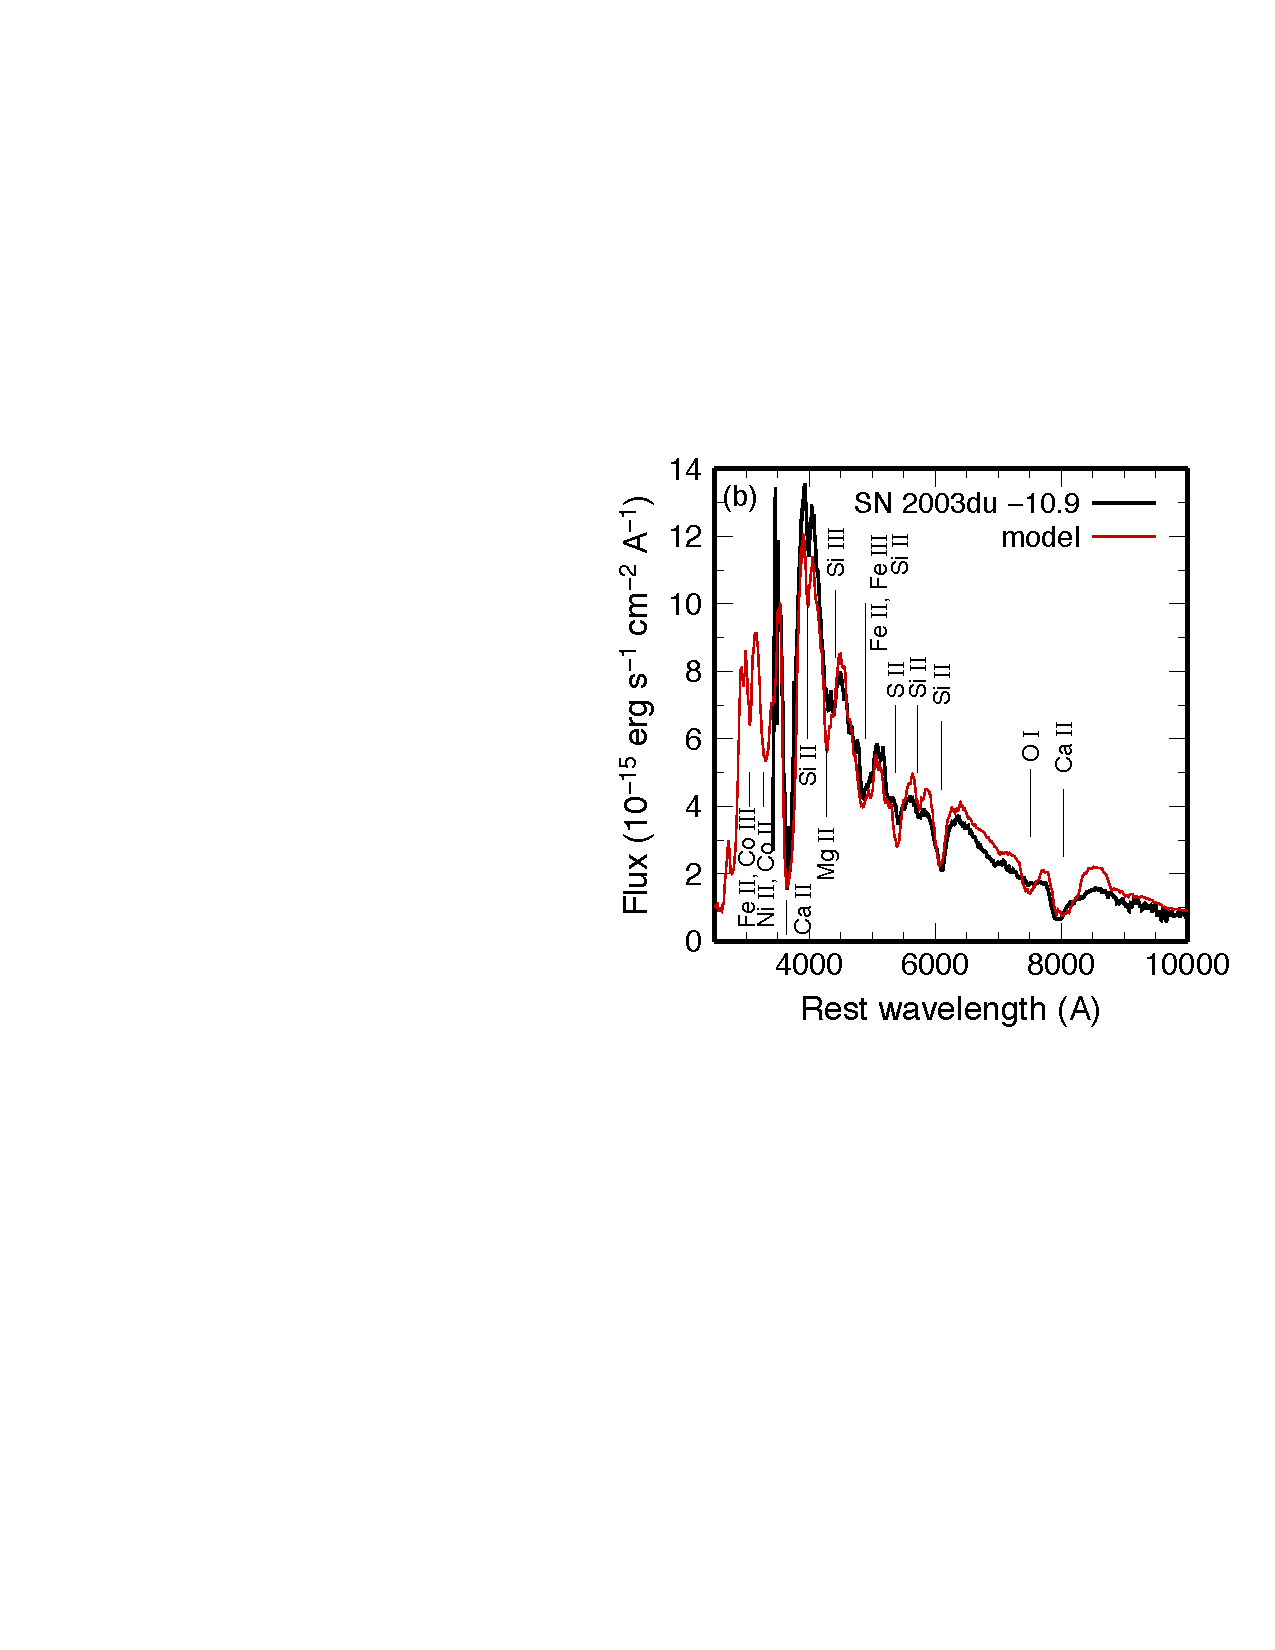
\includegraphics[width=0.45\textwidth]{chapter_intro/plots/sn2003du_t-10.pdf}}%
    \subfloat[SN2003du spectrum at maximum light. The light in the UV is being supressed and fluoresced into the red part of the spectrum.]{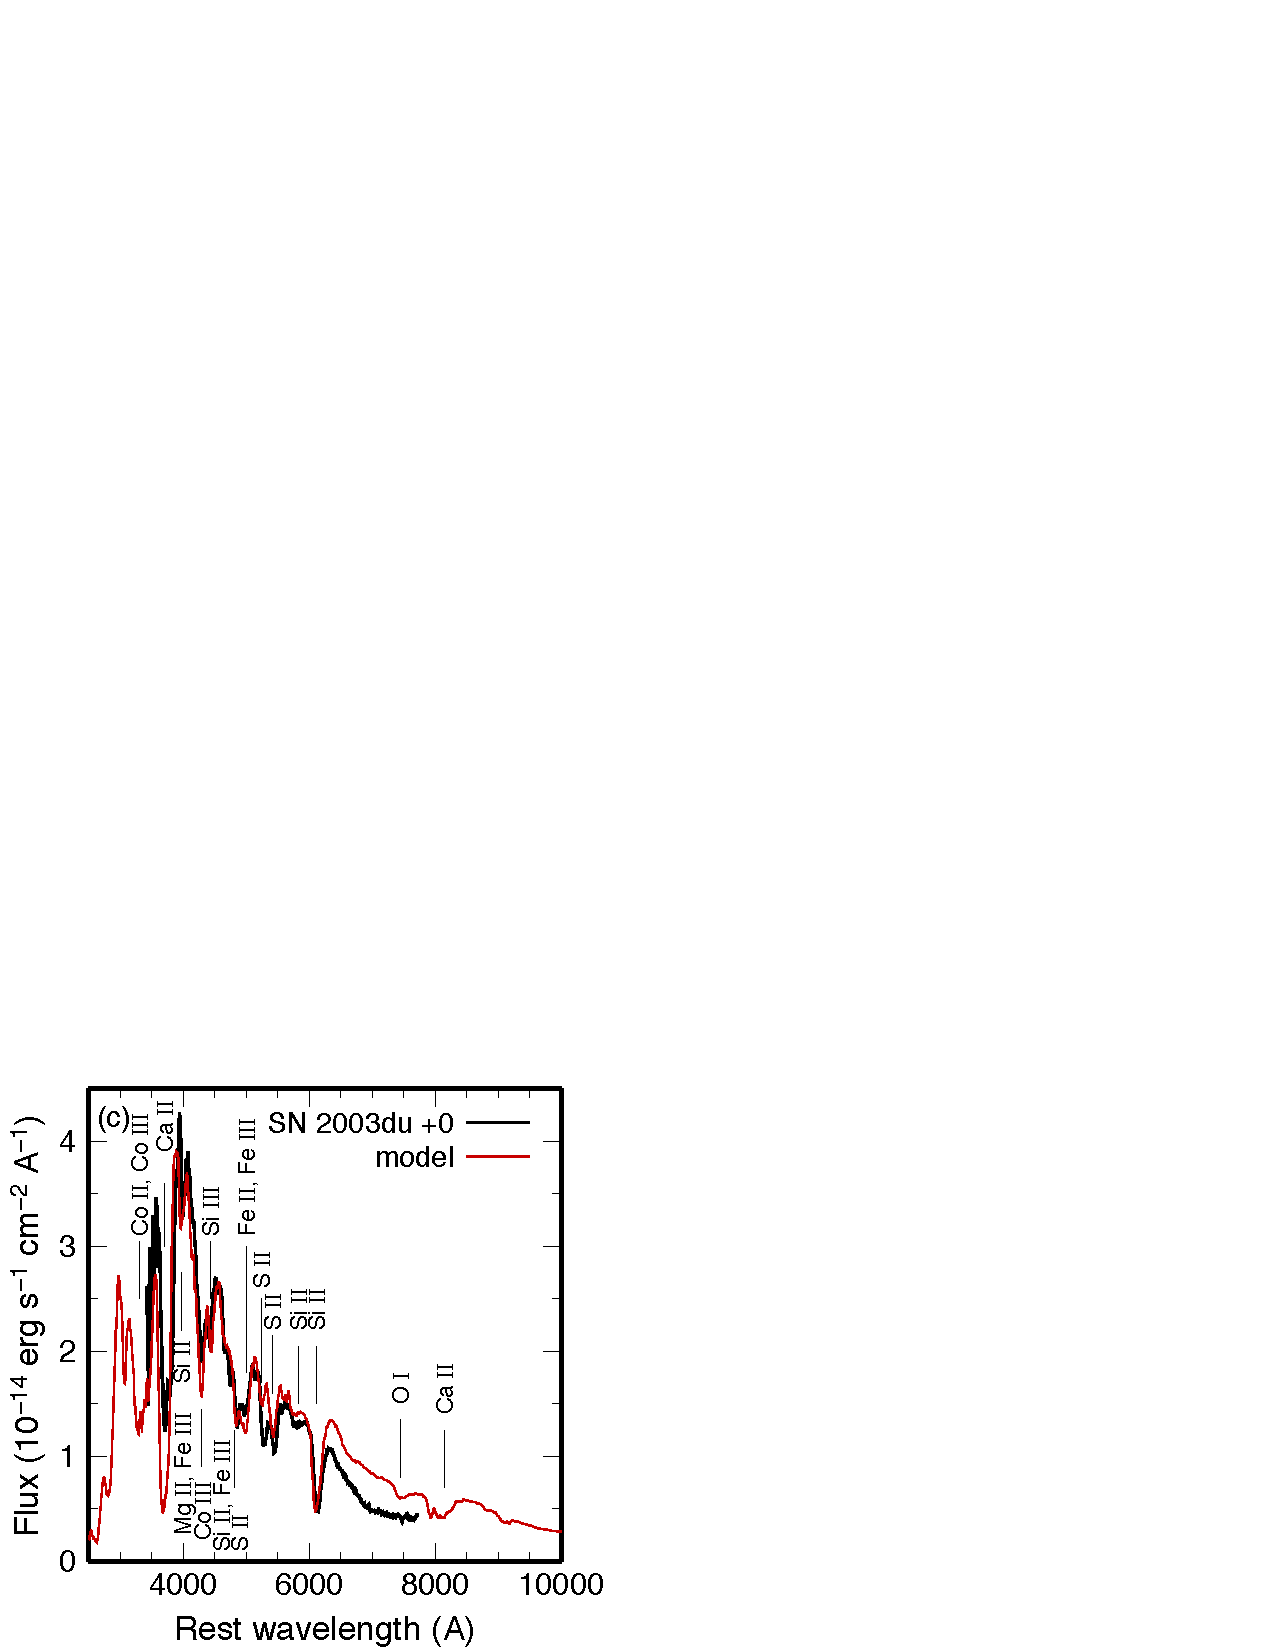
\includegraphics[width=0.45\textwidth]{chapter_intro/plots/sn2003du_t0.pdf}}%
   \caption{Premaximum evolution of \sn{2003}{du} spectra from \cite{2011MNRAS.410.1725T}.}
   \label{fig:sn2003du_premax}
\end{figure}

The \ion{Ca}{2} line is very prominent in the blue and often shows extremely high velocities at early times (in \sn{2003}{du} $v \approx 25000$\,\kms). There have been multiple suggestion for the cause of this unusual velocity, including interaction with Calcium in the \ism\ or high-velocity ejecta blobs \citep{1999ApJ...525..881H,2004ApJ...607..391G,2004ApJ...601.1019T,2005ApJ...623L..37M,2006ApJ...636..400Q,2006ApJ...645..470T,2007A&A...471..527G}.
There is a strong \ion{Mg}{2} feature at 4200\,\AA\ which is contaminated by several iron lines. Silicon and Sulphur both have strong features 5640\,\AA (\ion{S}{2}) and at 6355\,\AA (\ion{Si}{2}). The strong Silicon feature is the trademark for \sneia.

It is believed that in these early phases one should be able to see Carbon and Oxygen from the unburned outer layers. There is the \ion{C}{2}-feature at 6578\,\AA\ but it is normally very weak (if visible at all). The Oxygen triple feature at 7774\,\AA\ is also seldom very strong.

\paragraph{Maximum Phase} As the supernova rises to the peak luminosity a large fraction of iron group elements (especially \Ni) is suppressing flux in the UV and reemitting it in the optical (see Figure \ref{fig:sn2003du_premax}). The silicon lines become narrower as the photosphere reaches material deeper in the remnant. The ratio of the Silicon lines \ion{Si}{2} 5972\,\AA\ and \ion{Si}{2} 6355\,\AA\ is a good indicator for temperature \citep{1995ApJ...455L.147N}. 


\paragraph{Post-Maximum phase}
The contribution from iron-group elements is still rising, while the photospheric velocity has decreased to less than 10000\,\kms (see Figure \ref{fig:sn2003du_t+17}). The strong Calcium feature at 4000\,\AA\ is starting to disappear. 

\begin{figure}[htbp] %  figure placement: here, top, bottom, or page
   \centering
    \subfloat[SN 2003du 17 days past maximum light. The contribution of \ige is still rising.]{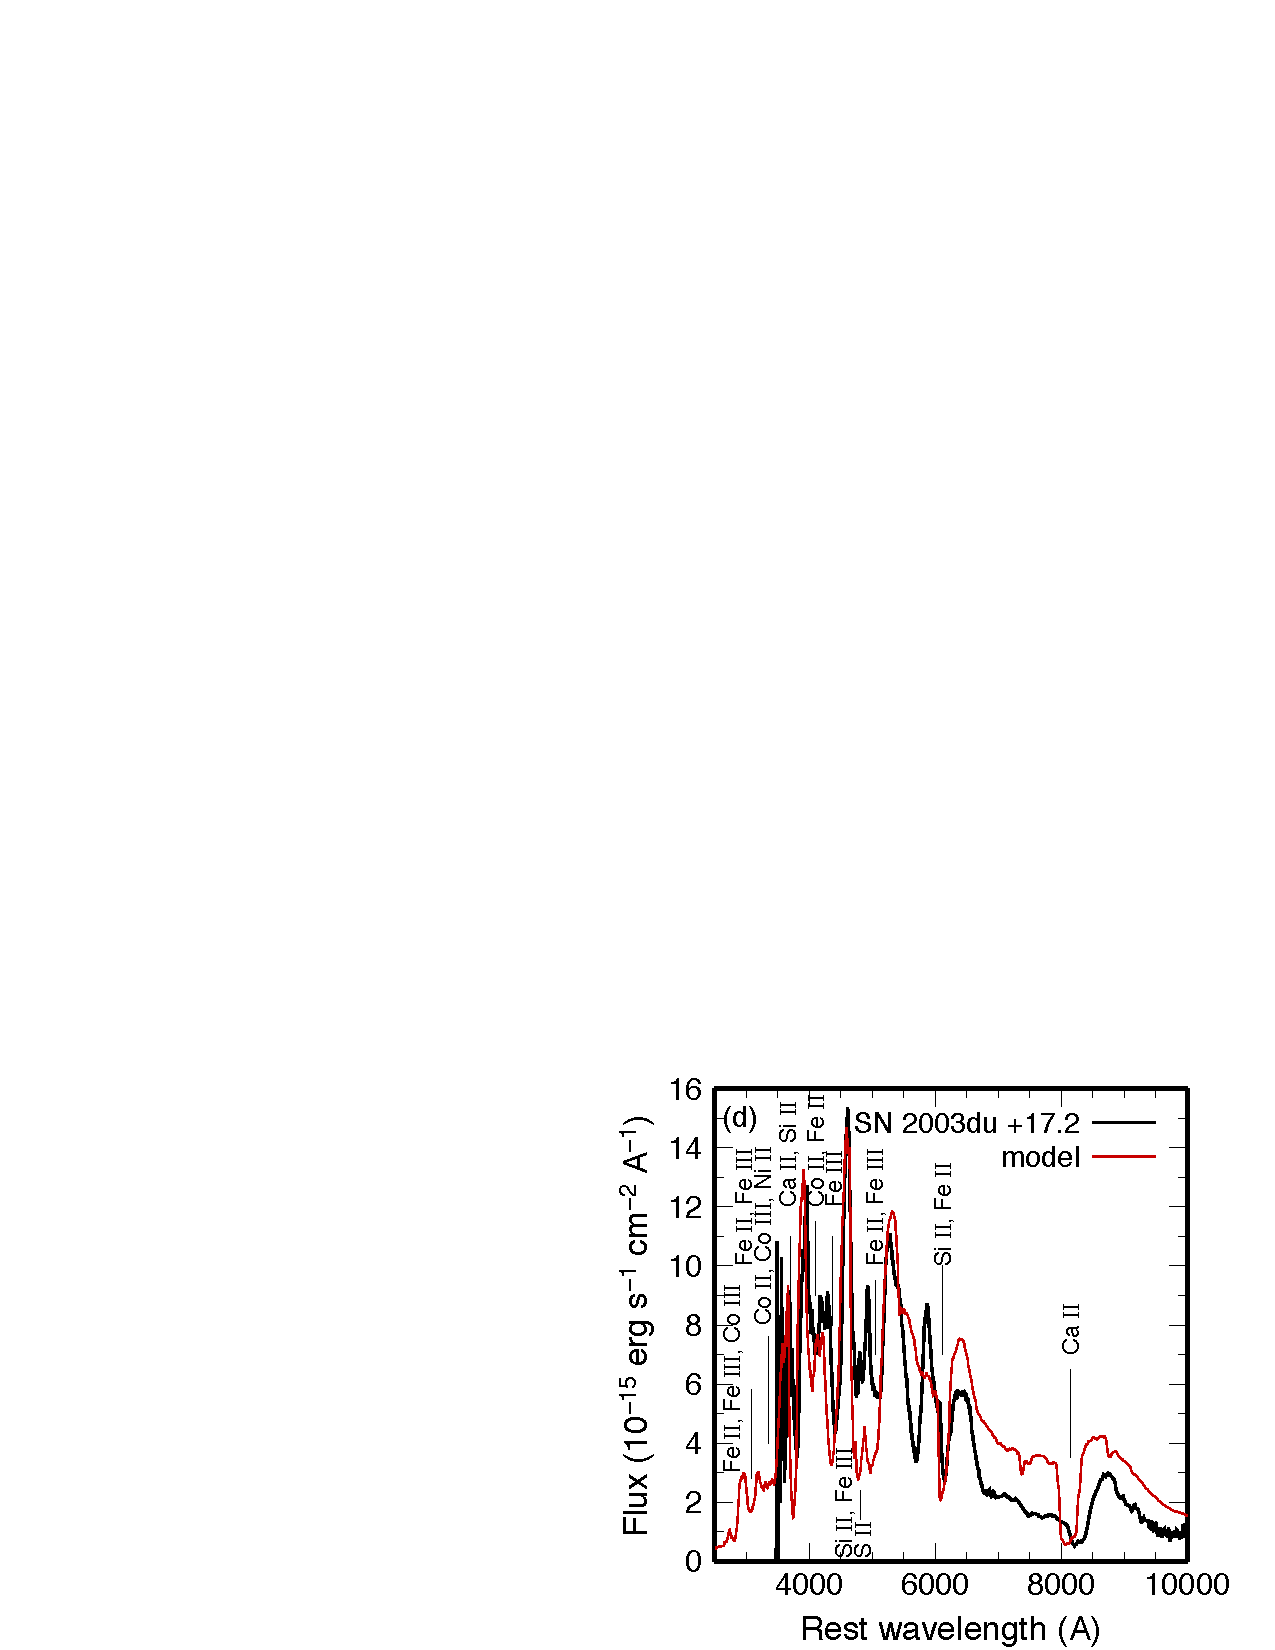
\includegraphics[width=0.45\textwidth]{chapter_intro/plots/sn2003du_t+17.pdf}} 
   \subfloat[In the nebular phase strong emission lines are visible. This phase is not observed very often but contains crucial information about the explosion physics.]{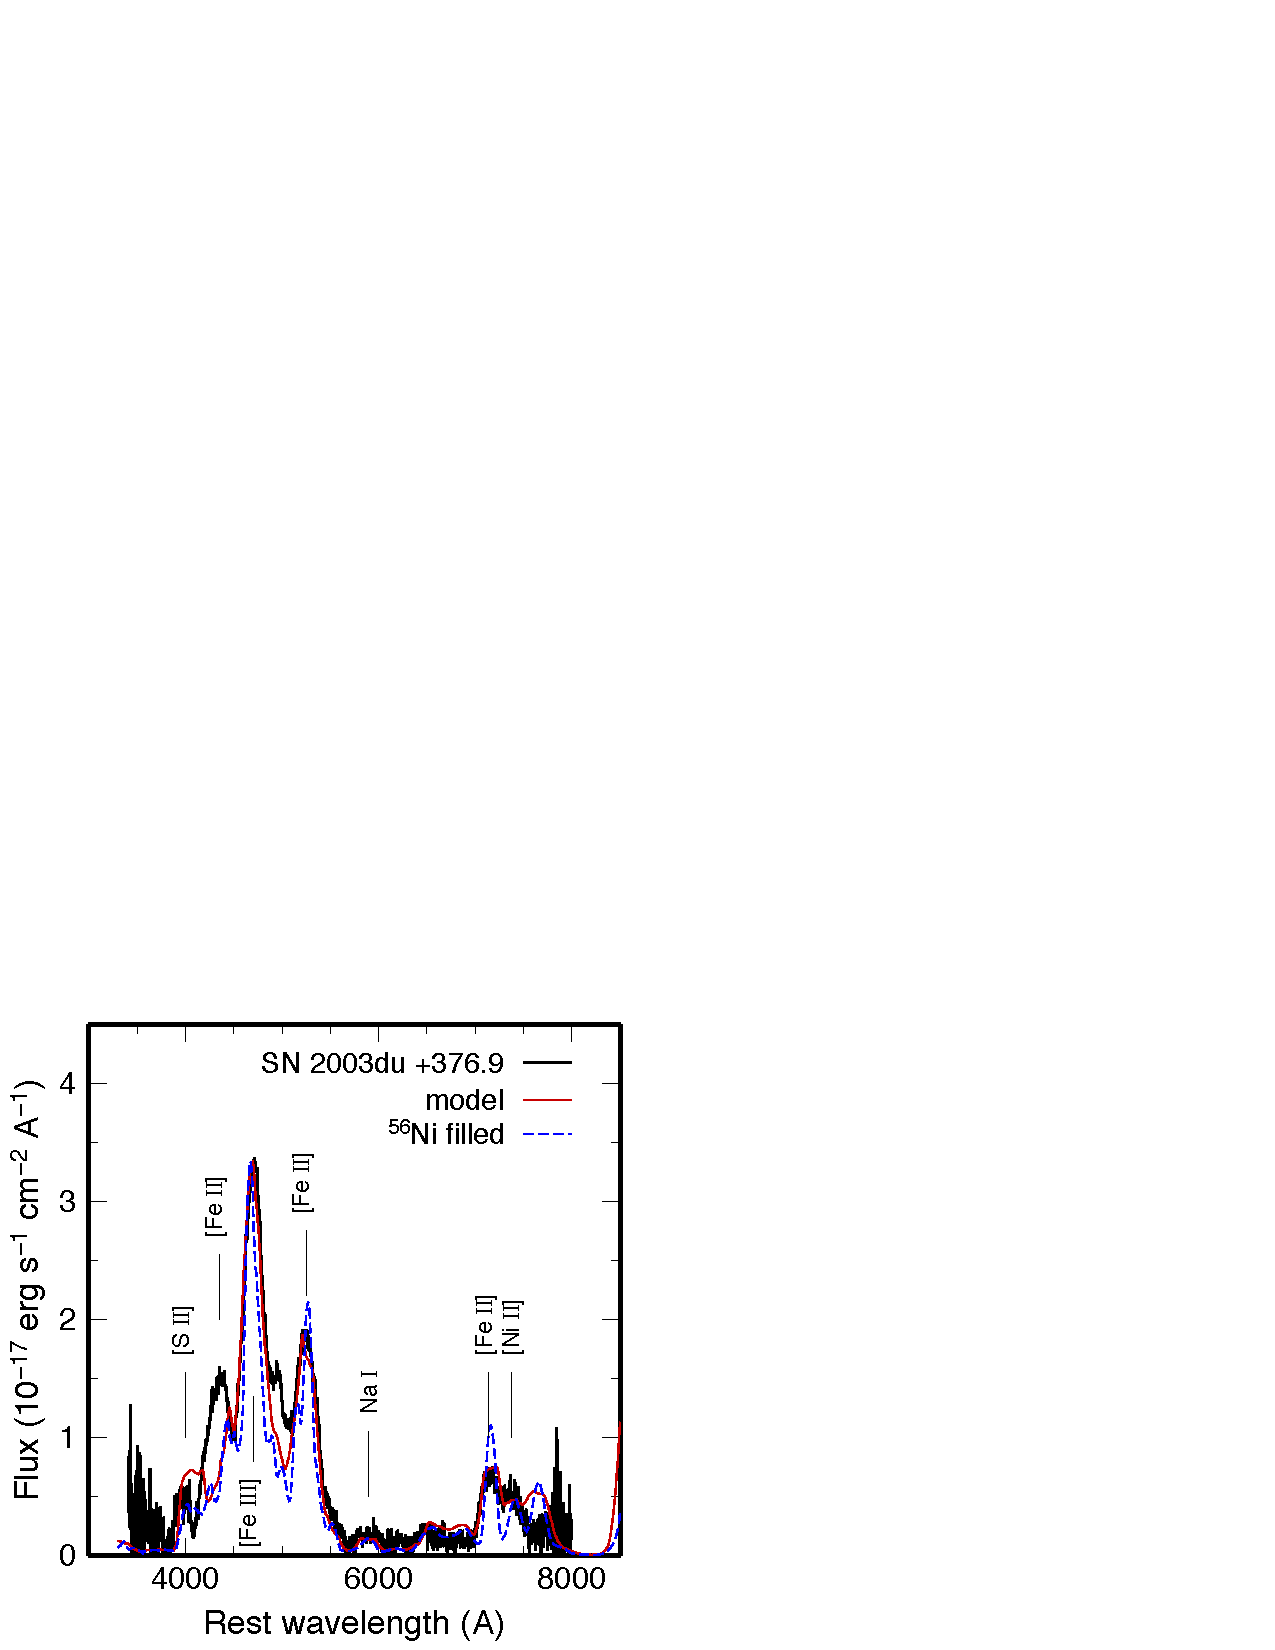
\includegraphics[width=0.45\textwidth]{chapter_intro/plots/sn2003du_nebular.pdf}}
   \caption{Postmaximum evolution of SN 2003du from \cite{2011MNRAS.410.1725T}.}
   \label{fig:sn2003du_t+17}
\end{figure}

\begin{figure}[htbp] %  figure placement: here, top, bottom, or page
   \centering

   \caption{example caption}
   \label{fig:sn2003du_nebular}
\end{figure}



\paragraph{Nebular-Phase}
As the supernova fades, the photosphere disappears. At this stage the spectrum is now characterized by strong emission lines which are produced by the elements from the very core of the explosion (see Figure \ref{fig:sn2003du_nebular}). The velocity has fallen under 5000\,\kms. 




\subsubsection{SNe II Spectra}
\sneii\ show much more variation in their spectra for each object than \sneia\ . In this section we will only give a very general and brief overview over \sneii\ spectra and spectral evolution. 
Compared to \sneia\ the initial spectrum is a relatively undisturbed continuum (see \ref{fig:sn_class_spectra}). The only strong lines visible are those of Hydrogen and Helium which are the elements present in the envelopes of the progenitors. 
As the photosphere recedes into the core heavier elements like Oxygen, Magnesium and Iron become visible. 

The nebular spectra are characterized by $H\alpha$, Oxygen and Calcium emission lines. 

Most knowlege we have about all classes of supernovae we have obtained through optical spectroscopy and photometry. Panchromatic studies of supernovae have been done but are for the moment rare.

\subsection{X-Ray \& Radio observations}

Compared to the traditional optical astronomy X-Ray \& Radio are relatively new fields. The information carried in the very high and low frequency photons is invaluable to understanding various transient events. 

The long \grb-phenomenon has been suggested to be the relativistic jet launched in a \snibc. It is believed that \grb s are visible when this jet poins towards the observer (also known as on-axis). In their late phase \grb 's jet spreads and is thought to emit isotropically in radio. This radio glow should be visible to both on-axis and off-axis observers, but has so far only been observed on-axis . \cite{2006ApJ...638..930S} have tried to find this isotropic radio emission at late times on \snibc\ to see if they are off-axis \grb s. The study however remained inconclusive.

\sneii\ have long been theorized to emit \xray s at shock breakout \citep{1978ApJ...223L.109K,1974ApJ...187..333C}. To observe them is technically very challenging as the supernova needs to be detected very early on. SN2008D was serendipitously discovered by observation with the Swift \xray\ telescope. It was in the process of observing another supernova \sn{2007}{uy} in the same galaxy when  picked up an extremely luminous source \cite{2008Natur.453..469S}. Subsequent ground based follow-up revealed a brightening optical counterpart which turned out to be a \snibc. The \xray-flash was that of the theorized shock breakout of a supernova in a massive star.

\cite{2008Natur.451..802V} have suggested that they found the progenitor of the Type Ia SN 2007on in \xray s. The main caveat speaking against their find was the sizeable distance between the supernova and the \xray-source. Their technique however is promising. Following up \sneia\ in \xray-archives could detect potential \sneia\ progenitors in a pre-explosion \xray\ phase.

Radio and \xray\ observation of both kinds of supernovae are still in its infancy and will provide great help when solving the current mysteries surrounding all types of supernovae.

\subsection{Supernova Cosmology}
Early in the last century astronomers where trying to gauge our place in the universe. \citet{1929PNAS...15..168H} discovered that the Milky Way was not the only galaxy of the universe but found that there were several such galaxies much farther than previously suspected. He used, among other methods, the known intrinsic luminosity ($L_0$) of Cepheid variables and determined using the observed luminosity the distance ($L/L_0 \propto 1/r^2$).  In addition he found that galaxies that were further away had a higher velocity from the Milky Way than close galaxies. He suggested that the universe was in a state of constant expansion. Cepheids distance measurements are only possible for very close-by galaxies and astronomers were feverishly searching for brighter more precise distance probes (also known as standard candles). The discovery that supernovae are distant objects \citep{1934PNAS...20..254B} motivated many astronomers to try to standardize them \cite{1938ApJ....88..285B, 1960ZA.....49..201V, 1968AJ.....73.1021K, 1999ApJ...517..565P}. 

This culminated nearly 70 years later in another paradigm changing discovery. The accelerating expansion universe was discovered, using the same principal but much more advanced technology, by two teams \citep{1998AJ....116.1009R}. 
Since then other techniques have come to the same conclusion \cite[e.g.]{2011MNRAS.tmp..951B}.

\paragraph{\snii\ Cosmology}
\sniip\ have been first suggested as cosmological probes by \citet{1974ApJ...193...27K}. It is important for cosmological distance probes to know the intrinsic luminosity precisely. At the plateau-phase of the supernova, caused by the hydrogen-recombination,  the temperature is well known (T=5000\,K). In addition it is assumed that the supernova is in free expansion, thus a measurement of the velocity and an assumption of the initial radius results in a known radius. Assuming the supernova to be a blackbody during plateau-phase one can then calculate a luminosity using the radius and the temperature. \sniip\ as distance candles, however, are observationally expensive and not as accurate as \snia\ as standard candles (15\% error for \snii  vs 7\% error for \snia\ \citep{2006ApJ...645..841N}).

\paragraph{\snia\ Cosmology}
\sneia\ have been one of the most successful distance probes. It is believed that \sneia\ are the explosion of C-O white dwarfs. The brightness of these objects is powered by the decay of \Ni. The quantity of \Ni\ produced in the explosion can be gauged from the evolution of the light-curve which then in turn can be used to calibrate the intrinsic brightness (see Figure \ref{fig:normalized_lightcurve}).
In the late 1990s new detector technologies (CCDs), computing and new telescopes made it possible to measure the light curves of many \sneia\ accurately. 

The amazing discovery that both \citet{1998AJ....116.1009R} and \citet{1999ApJ...517..565P} made with \sneia\ was that the universe, in stark contrast to the earlier assumption, was expanding at an accelerating rate. 

\begin{figure}[htbp] %  figure placement: here, top, bottom, or page
   \centering
   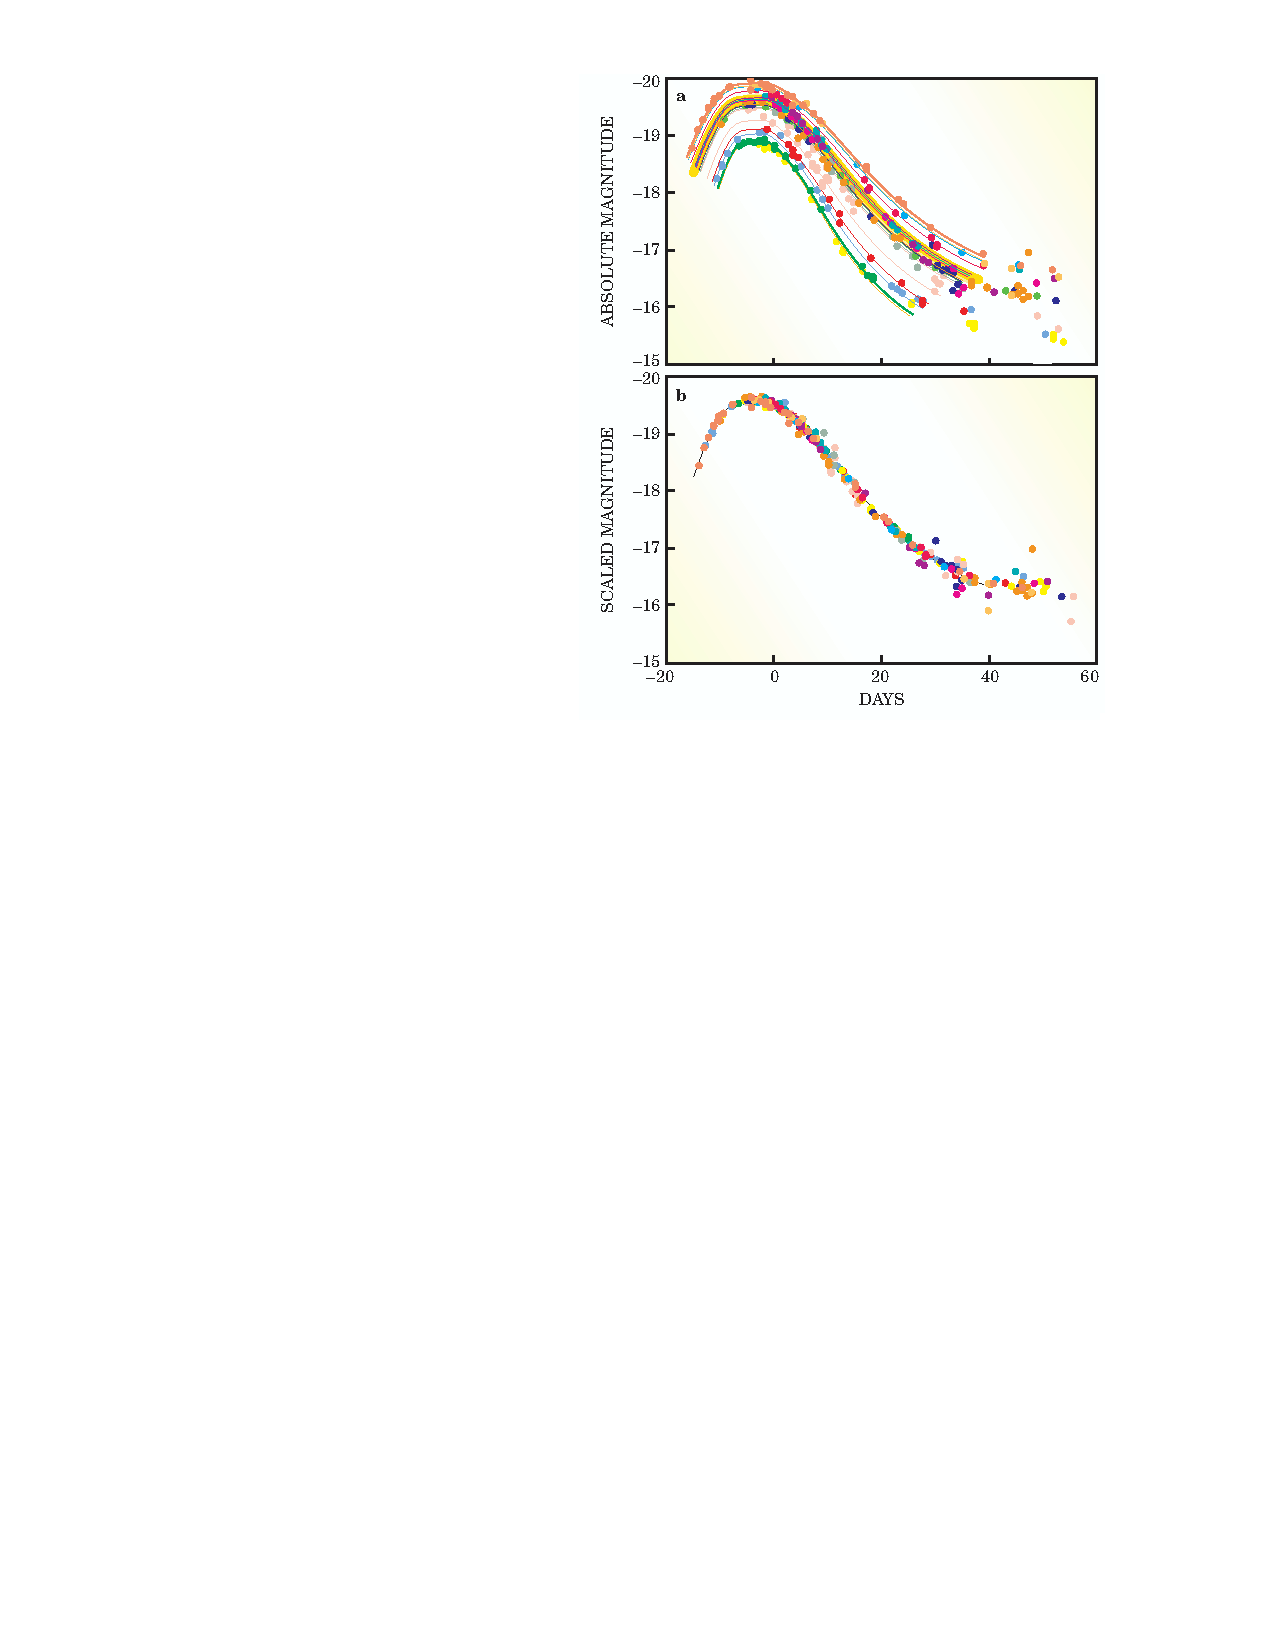
\includegraphics[width=0.7\textwidth]{chapter_intro/plots/lightcurve_scaled_perlmutter2003.pdf} 
   \caption{Replace with some data. any suggestions}
   \label{fig:normalized_lightcurve}
\end{figure}

\section{Post-explosion observations of Supernovae}

In most cases for \sneia, \sneibc\ and \sneii\ the distance to the supernova is too large to make detailed studies of these events post-explosion. 

When supernovae, however, happen in nearby galaxies or in our own. We have the chance of detailed post-explosion follow-up.
SN 1987A, which exploded in the close \lmc\, provided an ideal candidate for follow-up post-explosion which revealed that a previously observed Blue Supergiant was gone post-explosion \cite{1989A&A...219..229W}. This suggests that this star was the cause for the supernova. It was the first time a progenitor was identified with this ``direct detection''-method and since then many more progenitors have been unearthed post-mortem (for a review see 
\cite{2009ARA&A..47...63S}).

Modern X-Ray space telescopes provide data of exquisit detail to study the remnants of supernovae. Hydrodynamic and nonequilibirum ionization simulations of shocks from the supernova ejecta with the \ism\ can be used to measure temperature, elemental abundances and other parameters related to the state of the ejecta \citep{2003ApJ...593..358B, 2004AstL...30..737S, 2005ApJ...624..198B}. This technique of modelling has been used to scrutinize ancient remnants. Kepler and Tycho remnant have been unambiguously identified using \xray-spectroscopy to be remnants of \sneia\ \citep{2006ApJ...645.1373B, 2007ApJ...668L.135R}. This field is still at its infancy and future coupling of three dimensional models with \xray-observations will help reveal the explosions mechanisms for both physical types of supernovae: thermonuclear explosions and core-collapse of massive stars. 

Light-echoes are features that appear when light from a supernova scatters on dust in the \ism. This has been suggested by \citet{1940RvMP...12...66Z}, but only advancements in imaging techniques as well as digital processing made it possible to detect these echoes. \cite{2005Natur.438.1132R} pioneered this technique and found several of these echoes in the \lmc. Follow-up by \cite{2008ApJ...680.1137R} showed that it is possible to obtain a spectrum and identify the type of supernova with it. 
\cite{2008Natur.456..617K} subsequently observed the light-echo of Tycho's supernova (SN 1572) and identified it as a ``normal'' \snia and confirmed the previous \xray-spectroscopy result. Future wide-field surveys will hopefully reveal many more of these light-echoes. Light-echoes can not only be used for classification but also for a three dimensional spectroscopic view of supernovae \citep[demonstrated on the example of Cassiopeia A remnant][]{2011ApJ...732....3R}.

Post-mortem observations of supernovae and their light-echoes provide us with unique insights into these events. For nearby galaxies like the \lmc\ it is possible to scrutinize supernovae using their remnants and echoes which exploded over the last 20,000 years. This in turn can be used to infer rates and \dtd s \citep{2010MNRAS.407.1314M}.
\newpage
\section{Core-Collapse Supernova Theory}

All \snii\ and \snibc\ are believed to be powered by the collapse of the electron-degenerate iron core of massive stars. For the iron core to form there had to be several prior stages of evolution.

\subsection{Evolution of Massive Stars}  To understand the state of the star shortly before supernova evolution it is imperative to follow its evolution. For the topic of core-collapse we will concentrate on the nuclear physics of a single massive star evolution. There has been ample suggestions that some \snii\ and \snibc\ progenitors are binary \citep{1992ApJ...391..246P}, but their evolution is much more complex and is outside the scope of this work.  In this context massive stars are stars bigger than 8 \msun. This is the minimum mass for a star that is believed to explode in a \snii. Like all stars massive stars spend most of their lives on the main-sequence burning hydrogen. This happens via the carbon-nitrogen-oxygen cycle and its various side-channels (e.g $^{12}C(p,\gamma)\rightarrow^{13}N(e^+\nu)\rightarrow^{13}C(p,\gamma)\rightarrow^{14}N(p,\gamma)\rightarrow^{15}O(e^+\nu)\rightarrow^{15}N(p,\alpha)\rightarrow^{12}C$). For a 20 \msun star this phase lasts for 8.13 \myr (see \citet{2002RvMP...74.1015W}).

As the star evolves it begins to ignite Helium which burns via the triple-$\alpha$ process to Carbon ($3\alpha\rightarrow\Carb$) and then to Oxygen ($^{12}C(\alpha,\gamma)\rightarrow\Ox$). Table 1 in \citet{2002RvMP...74.1015W}) lists 1.17 \myr\ for this phase. 

Due to neutrino losses the stellar evolution is qualitatively different after helium burning. A neutrino-mediated Kelvin-Helmholtz contraction of the carbon-oxygen core describes the advanced stages of nuclear burning in massive stars (\citet{2002RvMP...74.1015W}). This contraction is occasionally delayed when the burning of new fuel sources counter-acts the neutrino losses. The star in the end is composited of a series of shells that burn the above fuel and deposit the ashes on the shell below (see Figure \ref{fig:fusion_shells}). There are four distinct burning stages. Their principal fuels are carbon, neon, oxygen, magnesium and silicon.

\begin{figure}[htbp] %  figure placement: here, top, bottom, or page
   \centering
   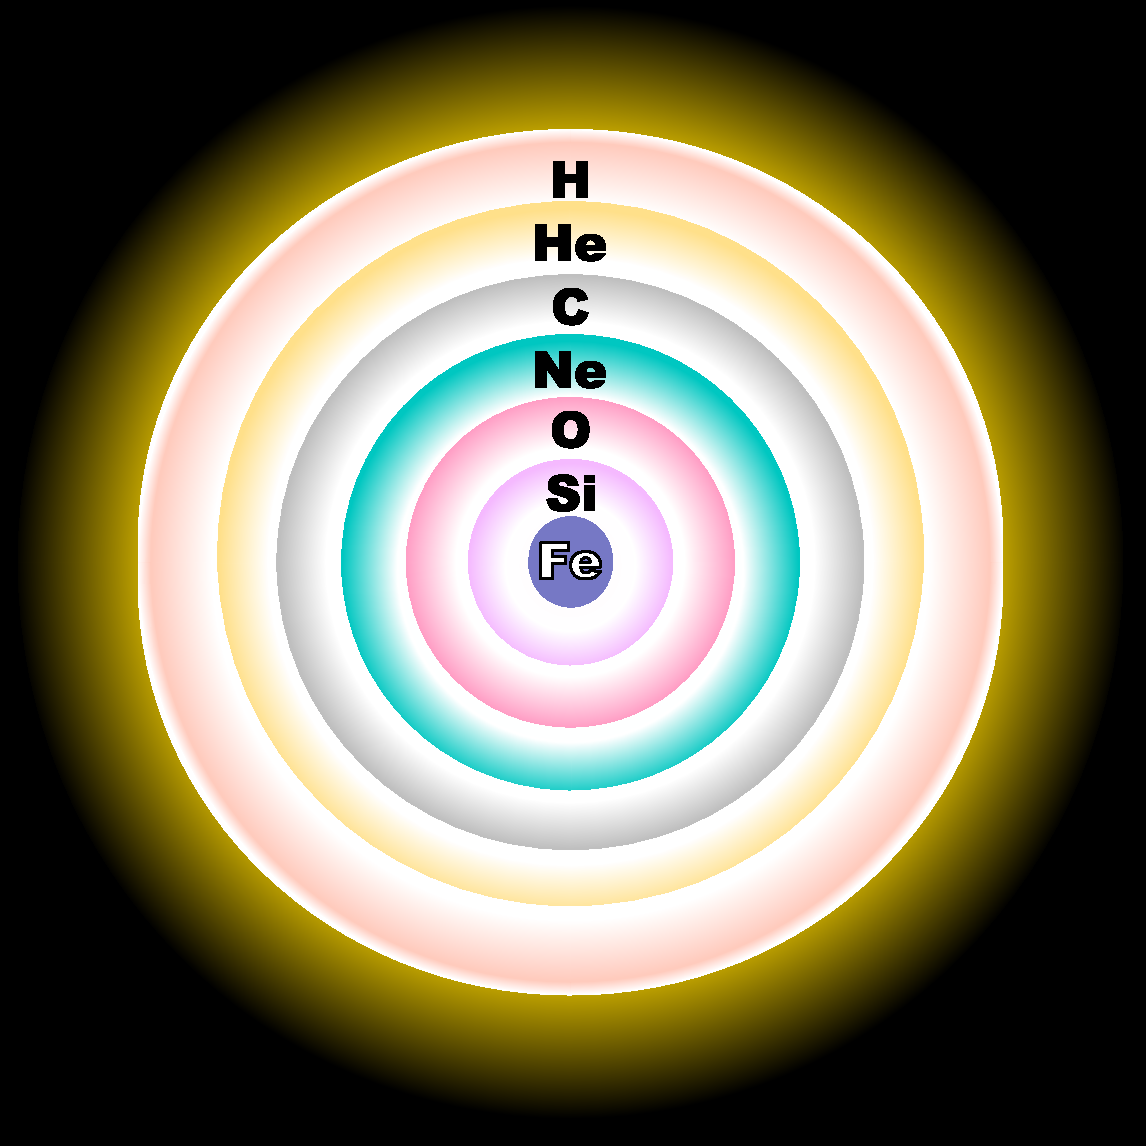
\includegraphics[width=0.5\textwidth]{chapter_intro/plots/fusion_shells.pdf} 
   \caption{Shell Burning of a massive star before \snii. (Source  Wikipedia, Creative Commons License)}
   \label{fig:fusion_shells}
\end{figure}


In the carbon burning stage two $^{12}$C nuclei are fused to an excited state of Magnesium which then decays slowly to $^{23}$Na (see Equation \ref{eqn:c_burning}).
\begin{eqnarray}
^{12}C+^{12}C\rightarrow^{24}Mg&\rightarrow&^{23}Mg+n \nonumber \\
	&\rightarrow&^{20}Ne + \alpha \nonumber \\
	&\rightarrow&^{23}Na +p \nonumber \\
	\label{eqn:c_burning}
\end{eqnarray}

Although oxygen has a lower Coulomb barrier, the next nucleus to burn after Carbon is Neon. This layer is composed of of  $^{16}$O, $^{20}$Ne and $^{24}$Mg and burns Neon with high-energy photons from the tail of the Planck distribution ($\rm ^{20}Ne(\gamma,\alpha)^{16}O$). 

In the next shell there is a composition of mainly $^{16}$O, $^{24}$Mg and $^{28}$Si. The bulk nucleosynthetic reaction is shown in Equation \ref{eqn:c_burning}. 

\begin{eqnarray}
^{16}O+^{16}O\rightarrow^{28}Si&\rightarrow&^{31}S+n \nonumber \\
	&\rightarrow&^{31}P + p \nonumber \\
	&\rightarrow&^{30}P + d \nonumber \\
	&\rightarrow&^{28}Si + \alpha \nonumber \\
	\label{eqn:c_burning}
\end{eqnarray}

The last shell is burning $^{28}$Si to $^{56}$N. The obvious reaction $^{28}\textrm{Si}+^{28}\textrm{Si}\rightarrow^{56}\textrm{Ni}$ does not take place, but is replaced by a very complex network of isotopes to burn to $^{56}\textrm{Ni}$. In simulations this is computationally intensive and numerically unstable (e.g .  \citet{1978ApJ...225.1021W} who carry a 128-isotope network). 
Following silicon burning the composition consists of mainly iron-group nuclei. 
At the end of silicon burning we are reaching nuclear statistical equilibrium. 

\subsection{Core collapse} Before the collapse,  the core consists of iron peak elements. Neutrino losses during carbon and oxygen burning decreased the central entropy sufficiently so that the core becomes electron degenerate. Such a degenerate core, which is higher than the Chandrasekhar mass (adjusted for Y$_e$, entropy, boundary pressure and other parameters) will collapse. 

There are two main instabilities that facilitate the collapse. As the density rises the Fermi-Energy becomes high enough for electrons to capture onto iron-group nuclei. This capture process removes electrons that were providing degeneracy pressure and reduces the structural adiabatic index. 

The second instability is the rise to temperatures where the nuclear statistical equilibrium favours free $\alpha$-particles. The collapse eventually leads to nuclear densities, the hard-core potential acts as a stiff spring during the compressive phase. It stores up energy and eventually releases this energy resulting in a "core bounce".  
\citet{1985PhRvL..55..126B,1987PhRvL..59..736B} believed the core bounce to provide the energy for the ensuing supernova explosion. More recent simulations however show that the bounce shock is not sufficient for a \snii\ explosion. The bounce shock looses energy by photo disintegrating the nuclei it encounters (loosing roughly $10^{51}$\,\erg\ per 0.1\,\msun).

The energy for a successful explosion is now thought to come from neutrino energy deposition. This reinvigorates the shock and leads eventually to an explosion which ejects the envelope of the massive star. \cite{2007ApJ...655..416B} suggest that instead of neutrinos, acoustic waves might heat up the ejecta and cause the explosion. In any case a newly born neutron star is left behind.

The precise explosion mechanism is unknown. Using progenitor models with different parameters like rotation and mass lead to different outcomes. \citet{2002RvMP...74.1015W} provide a very comprehensive review of the theory of evolution and core collapse. In particular they go into more detail describing the scenarios after core-bounce.

\subsection{Pair instability}
One alternate explosion scenario is the pair-instability supernova. This scenario is believed to only happen in stars with a helium core of more than 40\,\msun. After core helium burning the star starts to contract at an accelerated rate. The energy release during this process is used to produce electron-positron pairs rather than raising the temperature. If significant densities are reached, oxygen fusion eventually halts the implosion and the collapse bounces to an explosion. For very high stellar masses it is believed that oxygen fusion does not provide enough energy to halt the contraction and the star collapses to a black hole.


\subsection{Type II Supernovae}
The observables of these stellar cataclysm are the light curve, spectra and for one case even the neutrino wind. The supernovae goes through three distinct phases which can be observed. 

The shock-breakout is the first visible signal from the supernova.  \cite{1992ApJ...393..742E} calculated a duration for the  shock breakout of SN1987A to 180\,s three minutes, its  luminosity of $5\times10^{44}$\erg\,s$^{-1}$. 
Thus far it has been observed only once in 2008D \citep{2008Natur.453..469S}. They report a duration of 400\,s with a luminosity of $6.1\times10^{43}$\erg\,s$^{-1}$.

The plateau seen in many \snii\ (see Figure \ref{fig:snii_lc}) is produced by the recombination of hydrogen when hydrogen-rich zones cool to less than 5500\,K. The radiation comes effectively from a blackbody, whose luminosity is determined  by the radius of the photosphere.
Supernovae of Type IIL do not show this behaviour and are thus thought to have no or a very small hydrogen envelope.


After the recombination of hydrogen the light-curve drops off linearly and we see radioactivity providing the main energy source. \Ni\ decays to \Co\ with a half-life of 6.1\,d and then further to \Fe\ with a half-life of 77\,d. Most of the energy of the \Ni\ decay is used to accelerate the expansion of the core. The tail of the light-curve after the plateau is mainly powered by the decay of \Co. Some light be also produced by shock interaction with the \csm.





\subsection{Type Ib/c supernovae}
If the star lost all of its hydrogen envelope prior to core-collapse there is no plateau visible in the light-curve. Instead the light-curve is powered by radio-active decay after shock breakout. In addition, the hydrogen lines are not visible in the spectrum. This leads to the supernova being classified as Type Ib. If both hydrogen and helium envelopes are lost then the supernova is classified as Type Ic. 
This loss of envelope is presumed to be caused by stellar winds or binary interactions \citep{1992ApJ...391..246P}. 


\section{Thermonuclear Supernova Theory}
In this section we will discuss the theory of \sneia\ which are thought to be thermonuclear explosions of degenerate Carbon/Oxygen matter. The different progenitor scenarios leading to an explosion of a massive white dwarfs are discussed in Section \ref{sec:snia_progenitor}.

\subsection{White Dwarfs}
\label{sec:white_dwarfs}
Carbon/Oxygen white dwarfs are thought to be the progenitor stars of \sneia. White dwarfs are among the few stellar objects that do not hold hydrogen. This would explain the lack of hydrogen in \snia-spectra. It is general believed in the community that these objects accrete matter (for the possible scenarios see section \ref{sec:snia_progenitor}) until they get close to the Chandrasekhar-mass \citep[henceforth \mchan;][]{1931ApJ....74...81C}. It is a delicate balance between the ignition point that results in the thermonuclear run-away and the Chandrasekhar threshold which leads to a collapse of the star to a neutron star.
 
There are three main classes of white dwarfs: Helium, Carbon/Oxygen (henceforth \cowd) and Oxygen/Neon (henceforth \onemgwd) white dwarfs. Helium white dwarfs would start burning their Helium to Carbon and Oxygen well before it gets near the Chandrasekhar mass. In addition, these objects can also be ruled out as progenitors for \sneia\ as copious amounts of \ige\ produced in \sneia\, which are not consistent with the burning of a Helium white dwarf. 

The ultimate fate of an \onemgwd\ is thought to be the collapse into a neutron star. Once the \onemgwd\ is heavy enough electron capture begins in the core ($\Ne(e^-,\nu)\F[20](e^-,\nu)\Ox[20]$). Heating by the resulting $\gamma$-rays starts explosive Oxygen burning. However, the electron-capture is much faster than the Oxygen burning and promotes the collapse to a neutron star \citep{1991ApJ...367L..19N, 2005A&A...435..231G}. 

The favoured progenitor for a \snia\  are \cowd s. Most of these objects are born, however, with a mass around 0.6 \msun\ \citep{2007MNRAS.375.1315K}. It is thought that they accrete mass until they are getting close to the Chandrasekhar mass and then explode as a \snia.

\subsection{Pre-supernova evolution}
The white dwarf gradually accretes more and more material. Close to \mchan mild carbon burning ensues
\begin{align}
\nonumber
\Carb(\Carb,p) &\rightarrow \Na \\  \nonumber
\Carb(\Carb,\alpha) &\rightarrow \Ne \\ 
\Carb(\Carb,n) &\rightarrow \Mg[23]
\end{align},
but is mediated by photon and neutrino loses \citep{2005NuPhA.758..463L, 2007nps..book.....I}. As the cooling processes become less effective convection starts in the core. The energy output in the core increases. At this stage the thermal structure is largely controlled by Urca pairs. These reaction pairs consist of alternating electron captures and $\beta^-$\,-decays involving the same pair of parent and daughter nuclei. Two prominent examples which are important in pre-supernova evolution are \Ne[21]/\F[21]:
\begin{align}
\nonumber
\Ne[21](e^-, \nu) &\rightarrow \F[21] \\
\F[21](\beta^- \nu) &\rightarrow \Ne[21]
\end{align}
These processes can lead to either cooling or heating. \cite{2005NuPhA.758..463L} have modelled this process in a convective core. 

Ultimately, the pre-supernova evolution is hard to model theoretically as it is likely to be nonlocal, time-dependent, three dimensional and stretches over hundreds of years. The exact conditions at the time of explosion are therefore unknown. All explosion models have to assume simple initial conditions. 

\paragraph{Ignition}
The \urca processes will dominate core evolution for the last thousand years until explosion. As the temperature rises to $T\approx7 \times 10^8$\,K \citep{2000ARA&A..38..191H} the convection time ($\tau_c$) increases and becomes comparable to the burning time ($\tau_b$). Consequently the convective plumes burn as they circulate. Once the temperature reaches $T\approx 10^9$\,K $\tau_b$ becomes very small compared to $\tau_c$ and Carbon and Oxygen essentially burn in place. 
This is the moment of ignition. As the convective plumes burn while they rise it is likely that the initial flame seed does not start in the center of the core. \cite{2005A&A...431..635R} have used multiple flame seeds in their three dimensional full star models.

\paragraph{Thermonuclear Explosion}
From this point, initially there were two main options. The first option was the complete detonation (supersonic flame front) of the \cowd\ \citep{1969Ap&SS...5..180A}. It was quickly, discovered, however that this method burns to \nse\ and thus produces no \ime. These \ime\ are observed in \snia.

For a long time it was then suspected that the star instead of detonating would deflagrate (subsonic flame wave, mediated by thermal conduction). The fuel in front of the deflagration gets rarified by the energy from the flame. Hot light burning bubbles rise into the cold dense fuel and create Rayleigh-Taylor instabilities (see Figure \ref{fig:snia_ddt_roepke2007} at t=0.72\,s). 
Once the deflagration wave has run through the star, the resulting production of \Ni[56] is not enough to explain the light curve of normal \snia. The deflagration produces roughly 0.3\,\msun of \Ni[56], to power the light curve of normal \sneia\ one needs 0.6\,\msun \citep{2007Sci...315..825M}.

The currently favoured scenario is the one of delayed detonation. The star initially burns like in the deflagration scenario, then inhomogeneities in the deflagration front produce hotspots. In these hotspots the temperature gradients are so high that detonation waves form. The ensuing detonation front can only burn the cold unburnt-fuel and does not penetrate the ashes of the deflagration. Figure \ref{fig:snia_ddt_roepke2007} shows clearly how the detonation wave wraps around the cold ashes over the course of the detonation.


\begin{figure}[htbp] %  figure placement: here, top, bottom, or page
   \centering
   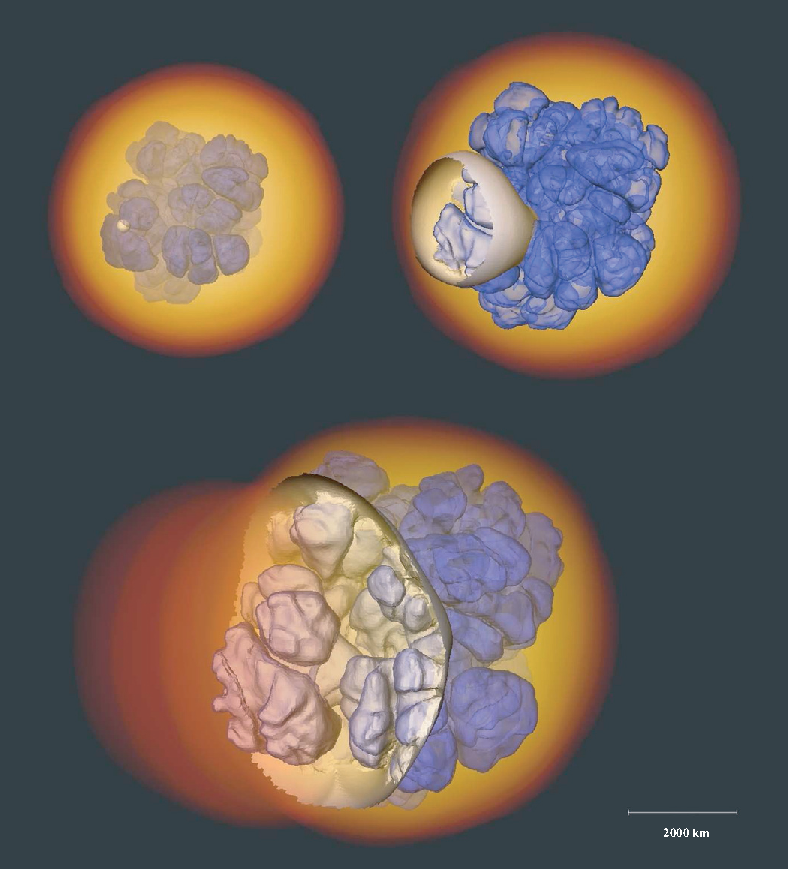
\includegraphics[width=0.7\textwidth]{chapter_intro/plots/ddt_roepke08.pdf}
   \caption{ Delayed detonation simulation from \citet{2008NJPh...10l5009R}. The upper panels show the deflagrated interior (marked in blue) and the detonation ignition point (small white sphere). The detonation wave wraps around the deflagration ash and consumes the cold fuel. (Image reproduced with kind permission of Fritz R\"{o}pke)}
   \label{fig:snia_ddt_roepke2007}
\end{figure}

An open question is if and how these transitions from deflagration to detonation occur in \sneia. This scenario reproduces the light curves and spectra reasonably well \citep{2009Natur.460..869K}. 


\paragraph{sub-Chandrasekhar-mass detonations}
\label{sec:subchandra}
\citet{1992ApJ...386L..13S} and \citet{2010ApJ...714L..52S} have explored the detonation of \cowd s at sub-Chandrasekhar masses.  \citet{2010ApJ...714L..52S} show that the detonation of a sub-Chandrasekhar-mass \cowd\ reproduce observed light-curves and early-time spectra of \sneia\ fairly well.

The main issue in this scenario is the ignition. \cite{2010A&A...514A..53F} have suggested an explosion mechanism in which a surface detonation of a Helium shell drives a shock-wave into the core. In the core this shockwave triggers an ignition by compression.  As an initial model they use a \cowd\ accreting from a helium rich companion building a thin helium shell around its CO interior \citep[described in][]{2007ApJ...662L..95B}. This helium shell is ignited and sends out a shockwave. As the helium flame spreads on the shell around the star it sends a shockwave into the core. Once 
the shockwaves converge off-center they create a the right environment for the ignition of a detonation wave (see Figure \ref{fig:subch_fink2010}.) 

This scenario reproduces the intrinisic luminosity variability in the class of \snia\ as each exploding white dwarf can have a different mass. 

\begin{figure}[htbp] %  figure placement: here, top, bottom, or page
   \centering
   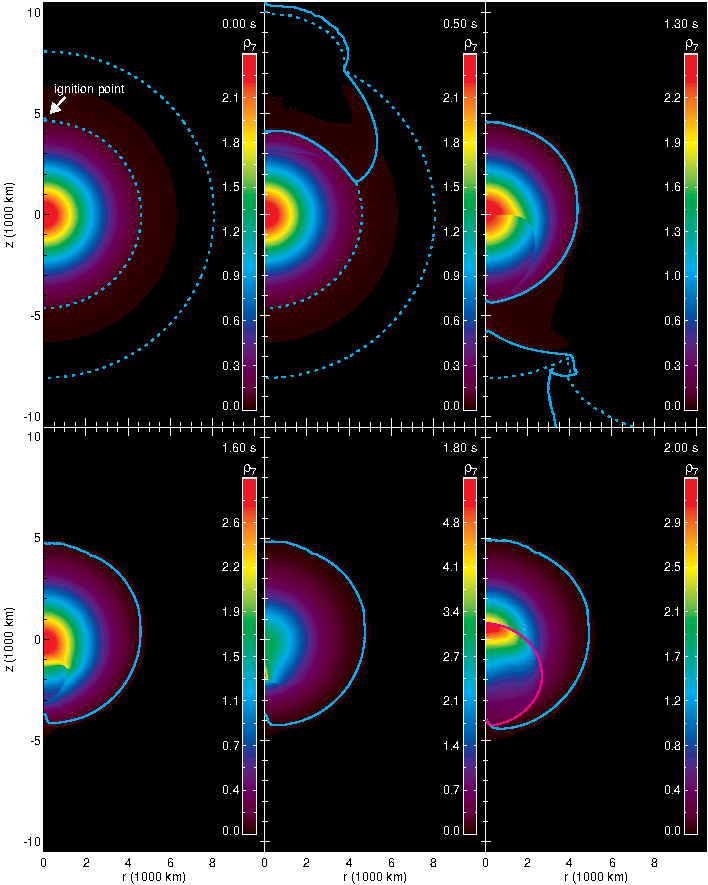
\includegraphics[width=0.7\textwidth]{chapter_intro/plots/fink2010.pdf} 
   \caption{The ignition point of the helium shell is marked in the upper left image. We can follow the helium shell sending shock waves into the core of the white dwarf. They converge in the lower left image at the opposite site of the Carbon/Oxygen core \citep[data from][figure kindly provided by Michael Fink]{2010A&A...514A..53F}. }
   \label{fig:subch_fink2010}
\end{figure}

\paragraph{\WD-\WD\ mergers}
\cowd\ mergers for a long time were thought to lead to a gravitational collapse \citep[same mechanism as the \onemgwd][]{1985A&A...150L..21S}. \citet{2010Natur.463...61P} has, however, successfully simulated the explosion of two merging \cowd s. The initial model was two equal mass 0.8\,\msun\ \cowd s. The merging process created a hotspot from which a detonation wave eminates. 
The resulting light-curves and spectra are faint and are similar to the class of sub-luminous \snia. 


\section{Progenitors of Type Ia Supernovae}
\label{sec:snia_progenitor}

\citet{1973ApJ...186.1007W} first introduced the modern binary evolution paradigm for \snia-progenitors. In their model a \cowd\ accretes matter from a red giant. A degenerate \cowd\ accreting from a non-degenerate companion is now known as the single degenerate scenario. 

\citet{1984ApJ...277..355W, 1984ApJS...54..335I} were the first to suggest that the merging of two \cowd s could also produce \sneia. This scenario is now commonly referred to as the double degenerate scenario.



\subsection{Single Degenerate Scenario}
The single degenerate scenario assumes a binary system with one evolved white dwarf and one non-degenerate companion. In most cases this non-degenerate companion is thought to be main-sequence to red giant. There are scenario that involve "exotic" companions such as helium stars. The companion (or donor) star is believed to have filled its Roche-Lobe and lose mass via Roche-Lobe-Overflow (henceforth \rlof).

\subsubsection{Accretion}
The main problem of the \sd-scenario is the accretion process.  As most white dwarfs are born with masses around 0.6\,\msun they need to accrete mass to reach the critical 1.38\,\msun. The process needs to be efficient as well as burn most accreted hydrogen to explain its lack in the spectrum.
 If the mass-accretion rate is too low it causes nova explosions which are thought to eject more mass than they had accreted prior \citep{Nomoto:1982p451}. There are however systems (e.g. RS Oph, U Sco) that have white dwarf masses close to 1.4\,\msun\ which have recurrent nova outbursts. It is very likely that these systems weren't born with a white dwarf that massive, but that these white dwarfs accreted the material. This suggest that despite nova outbursts efficient accretion is possible. 
 
 Too high accretion rates would engulf the binary in an extended red giant envelope which would promote a merger of the two compact objects. Debris of such an envelope is not seen in \snia-explosions. If To avoid this merger the system would have to loose the excess mass in a wind. This again results in a low accretion rate. There is only a very narrow range of accretion rates that allows the white dwarf to accrete hydrogen, stably burn it and efficiently accrete to \mchan. \cite{2004A&A...419..623Y} have suggest that rotation of the accreting white dwarfs might increase this very narrow parameter range.
 
A class of binaries called Supersoft X-Ray sources (\sss) might accrete hydrogen at a sufficiently high rate. At this rate Hydrogen and Helium burn hydrostatically, if retained, make these objects very strong contenders for \snia\ progenitors \citep[][and references therein]{2006astro.ph..6364D}. 
 
Another subclass of \sd-progenitors are AM CVn stars. These type of cataclysmic variable accretes from a helium star \cite{1992A&A...262...97V}. This scenario would very conveniently explain the lack of hydrogen in \snia-explosions. \citet[][]{2010A&A...514A..53F} have found a way that such systems can explode in a \snia (see Section \ref{sec:snia_theory}).


\subsubsection{Donor Stars}
The \sd-scenario requires a secondary companion (also known as donor) star. If this companion survives the explosion it would be a calling card for the \sd-scenario. 

\citet{2000ApJS..128..615M} have simulated the impact of \snia-ejecta on main-sequence, sub-giant and red-giant companion. In the case of the main-sequence companion the supernova ejecta heats a small fraction (1-2\%) of the envelope which is lost post-explosion. \citet{2008A&A...489..943P} have repeated the simulations for the main-sequence companion and find similar results, but suggest that less mass is lost. Post-explosion the star could be very luminous (500 -- 5000 \lsun). It is expected to cool down between 1400 -- 11000 yrs and follow the main-sequence track. 

For the sub-giant companion the simulations show very similar results to the main-sequence companion. In summary, the subgiant looses only a small fraction of the envelope (10 -- 15\%) and similar to the main-sequence star will be very luminous shortly after the explosion. After thermal equilibrium is established the companion will return to a post-main-sequence track. 

The case of the red-giant, however, is very different. \citet{2000ApJS..128..615M} suggest that it will loose most of its loosely bound envelope. Post-explosion the remaining core rises contracts and the temperature rises to more than $3 \times 10^4$\,K. The object may appear as an under luminous main-sequence O or B star. 


\cite{2009A&A...493.1081J} have suggested low-mass single white dwarfs to be the remaining cores of red-giant donor stars. This would result in a convenient explanation for the existence of these objects. 

One feature of surviving companions may be an unusually large rotational velocity post-explosion \citep[][chapter \ref{ch:sn1572_starg} of this work]{2009ApJ...701.1665K}. Due to tidal coupling during the \rlof-phase one calculate the expected rotational velocity from the escape velocity of the donor (see Figure \ref{fig:theorot}). Late-type stars usually don't display such high rotational velocities. Thus this feature is a very useful discriminant when looking for donor stars. 

Most simulations suggest that the donor-star would survive the explosion one way or another. There have been several attempts to find these objects in ancient supernova remnants. \citet{1980ApJ...241.1039S} found a OB subdwarf star located 2.5 \arcmin from the center of the remnant of SN1006 and suggested this as the donor star. Subsequent analysis by \cite{1997ApJ...477L..53W, 1983ApJ...269L...5W} have however revealed however strong red and blue shifted iron lines. The velocities of these lines are on order of 5000\,\kms which is the same as the velocity of the freely expanding remnant of \sn{1006}. This suggests the star to be located behind the remnant.
 
The search of donor stars in ancient remnants is one of the main parts of this thesis and we direct the reader to chapter \ref{chap:sn1572_starg} and chapter \ref{chap:sn1572_hires}.



\subsection{Double Degenerate Scenario}
\citet{1984ApJ...277..355W} and \citet{1984ApJS...54..335I} were the first to suggest merging white dwarfs as progenitors for \snia. There are several advantages to the \dd-scenario. For example, it naturally explains the lack of hydrogen in \snia-spectra. The accretion problem encountered in the \sd-scenario are also eleviated with \dd-scenario, as long as the sum of masses of both \cowd's is above \mchan. 

The problem, however, is that most \snia\ are relatively homogeneous. It is hard to reconcile this fact with the merger of two white dwarfs with different initial masses, composition, angular momenta and different impact parameters. Another caveat, however, is that the accretion of the disrupted lighter white dwarf onto the more massive white dwarf might lead to the transformation into a \onemgwd (see section \ref{sec:white_dwarfs})

\cite{2010Natur.463...61P} have simulated the merger of two equal-mass white dwarfs (0.8\,\msun) and conclude that the outcomes of these mergers might be subluminous \sneia.

In summary, mergers of white dwarfs might be able t explain some of \snia. It is however still debated if these events are responsible for the ``normal'' \sneia. 

\subsection{Constrains for different progenitor scenarios}

Radio observations in the case of \sneia\ can for example reveal the shock interaction of the ejecta with the \csm. The single degenerate scenario predicts more \csm than the double degenerate scenario. \citep{2011arXiv1105.6188H} have stacked radio observations of \sneia\ in the visibility plane. They can not detect any source. This could hint that the double degenerate scenario is the more common, but many caveats remain.

On the other hand however \cite{2007Sci...317..924P} have found variable Sodium features using high-resolution spectra of \sneia. These hint at the evolution of the Sodium ionization state in the \csm caused by the variable \snia\ radiation field. A wind from the donor star would provide material with the right geometric distribution to reproduce these features. Recently \cite{2011A&A...530A..63P} have seen similar features in the recurrent nova RS Ophiuchi. This could hint that recurrent novae with red giant donor stars might be responsible for some \sneia. 


\cite{2010ApJ...708.1025K} predict excess in UV flux in the \snia light curve at early times. This effect depends on orientation of the system to the line of sight and the state of the donor. The effect would be biggest for a giant donor. \cite{2010ApJ...722.1691H} do not see this excess in the SDSS supernova set. This suggests that the red giant channel is not common for \sneia\ and might suggest that \dd-scenario is predominent. There remain, however, many caveats. The orbits of the \sd-system might be closer than expected (suggesting that the existing light-curve data is not early enough) or the effect overestimated.

It remains a mystery that \sneia\ do not show lines of Hydrogen which might be expected from the wind or stripped envelope in the \sd-model. \citet{2007ApJ...670.1275L} have searched in the nebular spectra of two \sneia\ for hydrogen and place an upper limit of 0.1\,\msun\ for both these explosions. One might take this as a further hint against the \sd-scenario. On the other hand \citet{2011ApJ...730L..34J} suggest that a red giant donor could significantly shrink during the \rlof. This would place the the stripped hydrogen below the current detection limit. 

\cite{2010ApJ...719..474D} have not found enough \sss, which are suggested \snia-progenitors for the \sd-scenario. In addition, \cite{2010Natur.463..924G} have not found enough accumulated X-ray flux from elliptical galaxies if all \snia-progenitors were \sss\ (assuming the X-Ray flux calculated for these objects is correct). The main caveats are that the \snia-progenitors might only be in the \sss-phase for a moderate amount of time. In addition, these objects could be engulfed in a envelope, which would reprocess the produced \xray s to optical or infrared wavelengths.

Finding a donor star of the \sd-scenario in a \snr\ post-explosion, would resolve the question for the progenitor system at least in the searched remnant. The main work of this thesis investigates this technique and we will refer the reader to Chapters \ref{chap:sn1572_starg,chap:sn1572_hires, chap:sn1006}. 

Population synthesis together with observations of \dtd s are an important step in exploring the different progenitor scenarios. \citet{2008ApJ...683L.127H, Han:2004p444}  and suggest when compared to observations that the \sd-scenario is not far from explaining the observed \dtd\ (for references on \dtd\ see section \ref{sec:sn_rates}). 
\citet{2009ApJ...699.2026R, 2010A&A...515A..89M}, however, have explored the \snia-rate using several progenitor scenarios (\sd, \dd\ and \amcvn). Both suggest that the \sd-scenario on its own can not explain the observed \sneia-rate. The \dd-rate seems to be much closer to the observed frequency. Possibly a mix of all channels is required to explain the observed rate. 

In summary, the question of the progenitors is currently one of the most highly debated in \sneia\ research. There exist multiple arguments for both the \sd-scenario and \dd-scenario. In addition, new scenarios like the core-degenerate system in which a white dwarf merges with the hot core of a massive \agb\ star \cite{2011arXiv1106.2027I} are emerging. \cite{2011arXiv1102.4342D} and \citet{2011ApJ...730L..34J} suggest that the accreting white dwarf would be spun-up during accretion. The ignition of these highly spinning white dwarfs would be delayed and the companion might have time to evolve. This might possibly forfeit some of the arguments brought against the \sd-scenario. 
\cite{2010ApJ...722L.157V} on the other hand suggests the merger of two equal mass white dwarfs with a total mass less than \mchan. There remain still many caveats, but coupled with the work on sub-Chandrasekhar mass detonations by \citet{2010ApJ...714L..52S}, this might provide an interesting scenario. The main advantage is the predicted rate of these low-mass white dwarf mergers might be high enough to reproduce the observations.
More and novel observations of \sneia\ and \snr\ will hopefully help constrain the progenitor scenario. In the community some astronomers are now suggesting a multi-channel approach to explain \sneia\ phenomenon.
 

\newpage
\section{Thesis motivation}
One of the most pivotal moments in astronomy in recent years was the discovery of the acclerating expanding universe by \citet{1998AJ....116.1009R} and \citet{1999ApJ...517..565P}. This discovery catapulted \sneia\ into the limelight of the astronomical community. There has been many advances in recent years in the understanding of these cataclysmic events (explosion models, rates, etc.). One critical piece of the puzzle, however, has so far eluded discovery: The progenitors of \sneia. This work's main aim is to find evidence for one \snia-progenitor scenario. The \sd-scenario proposes a white dwarf accreting from a non-degenerate donor star. To the best of our knowledge this donor star is thought to survive the explosion and would be visible thereafter. We have tried to find this companion in two of three easily accessible ancient supernova remnants (SN1572 and SN1006). 
In chapter \ref{ch:sn1572_starg} we have obtained spectra of \starg\ which had been suggested as the donor star of SN1572 \citep{2004Natur.431.1069R}. Although we confirmed some of the suggested parameters we could not reproduce the unusually high radial velocity which led to the claim. 

We revisited SN1572 in chapter \ref{ch:sn1572_hires} with new observations of \starg\ and five other stars in the neighbourhood of SN1572. This resulted in \starg\ to be not a very viable donor star (it is hard to completely rule stars out). We discovered a curious A-Star located serendipitously right in the center of SN1572. Despite its bizarre parameters we could not reconcile this star (\starb) with any feasible progenitor model. We, however, found a scenario which explains \starb's features but does not involve it in SN1572. 

SN1006 provides a perfect opportunity to search for progenitor stars. It is the closest known remnant of a \snia\ (2\,kpc). We have obtained 80 spectra of stars close to the center of the remnant and present them in chapter \ref{ch:sn1006}. Again we did not find any obvious donor stars. 

We have obtained spectra of stars around SN1604 but these are not presented in this work.

Progenitor hunts provide us with information of the scenarios pre-explosion. Spectra on the other hand help to unravel the happenings during and post-explosion. \cite{2008MNRAS.386.1897M} have developed a code that can produce synthetic \snia-spectra from fundamental input parameters. Fitting an observed \snia\ is for the moment a manual task. This requires many days, if not weeks, of tweaking. The deluge of spectroscopically well-sampled \sneia\ from surveys is already hitting us. Manual analysis of all these spectra is impossible. The information about the explosion hidden in the spectra is, however, crucial to our understanding of these events. In chapter \ref{chap:dalek} we present our work towards automating this fitting process. We have tried a variety of algorithms to explore the vast and extremely complex search space. Working together with members of the computer science community we are exploring the use of genetic algorithms to solve this problem. 
This work is not finished yet, but we present preliminary methods in \snia-fitting in chapter \ref{chap:dalek}. Once finished we can apply this method not only in fitting \snia, but fitting other supernovae and in other areas of astronomy. 

In summary, this work explores two areas of supernova physics. The hunt for progenitors has not yielded obvious candidates, but may suggest a rethinking of the "normal" \sd-scenario. The automation of the supernova fitting is in its infancy stage. We have however shown that it is possible to explore the space in an automated fashion. This will hopefully yield abundances and energies for many thousand supernovae. 
The close collaboration with computer science community has shown how important cross-disciplinary research is in this era of science. 


